%% LyX 2.1.4 created this file.  For more info, see http://www.lyx.org/.
%% Do not edit unless you really know what you are doing.
\documentclass[12pt,english]{report}
\usepackage{charter}
\renewcommand{\familydefault}{\rmdefault}
\usepackage[T1]{fontenc}
\usepackage[a4paper]{geometry}
\geometry{verbose,tmargin=2.5cm,bmargin=2.5cm,rmargin=2.5cm}
\setcounter{secnumdepth}{3}
\setcounter{tocdepth}{3}
\setlength{\parskip}{\medskipamount}
\setlength{\parindent}{0pt}
\usepackage{color}
\usepackage{babel}
\makeatletter

\makeatother
\usepackage{float}
\usepackage{graphicx}
\usepackage{setspace}
\usepackage{nomencl}
% the following is useful when we have the old nomencl.sty package
\providecommand{\printnomenclature}{\printglossary}
\providecommand{\makenomenclature}{\makeglossary}
\makenomenclature
\onehalfspacing
\usepackage[unicode=true,
 bookmarks=true,bookmarksnumbered=true,bookmarksopen=true,bookmarksopenlevel=1,
 breaklinks=true,pdfborder={0 0 1},backref=false,colorlinks=true]
 {hyperref}
\hypersetup{
 linkcolor=black, citecolor=red, urlcolor=blue, filecolor=blue, pdfstartview=XYZ}

\makeatletter

%%%%%%%%%%%%%%%%%%%%%%%%%%%%%% LyX specific LaTeX commands.
%% Because html converters don't know tabularnewline
\providecommand{\tabularnewline}{\\}

%%%%%%%%%%%%%%%%%%%%%%%%%%%%%% User specified LaTeX commands.
% the pages of the TOC is numbered roman
% and a pdf-bookmark for the TOC is added
\pagenumbering{roman}

%\let\myTOC\tableofcontents
%\renewcommand\tableofcontents{%
 % \pdfbookmark[1]{\contentsname}{}
 % \myTOC
 % \cleardoublepage  }

%*****Chapter style******
\usepackage[Glenn]{fncychap}
\ChNameVar{\large}
\ChTitleAsIs
\ChTitleVar{\bfseries\Huge}

%*****Header style*******
\usepackage{fancyhdr}
 
\pagestyle{fancy}

\fancyhf{}
\fancyhead[LE,RO]{\thepage}
\fancyhead[RE,LO]{\footnotesize\nouppercase{\leftmark}}

%\renewcommand{\chaptermark}[1]{\markboth{#1}{}}

\renewcommand{\headrulewidth}{0,5pt}

%****Glossaire Title*****
\renewcommand{\nomname}{Glossaire}

\makeatother

\begin{document}
\noindent 
\begin{titlepage}
\begin{center}
% Upper part of the page
\begin{minipage}{0.4\textwidth}    \end{minipage}
\centerline{{{\fontfamily{cmr}  Academic year : 2018-2019}}}
%\begin{minipage}{0.4\textwidth} \begin{flushright} Academic year : 2018-2019 \end{flushright}\end{minipage}
\rule[0.5ex]{1\columnwidth}{1pt}\\[0.5cm]
\textsc{\large{University of Sousse}}\\
\textsc{\large{National School of Engineering of Sousse}}\\

\includegraphics[width=0.3\textwidth]{logo.pdf}\\[-0.5cm]
\Large{Graduation project report}\\[0.5cm]
\Large{ \bfseries{Applied Computer Engineering}}\\
\normalsize{Option: Distributed Systems}\\
~\\[0.6cm]
\rule[0.5ex]{1\columnwidth}{1pt}\\[0.5cm]
{ \huge \bfseries Designing and Developing a platform of remote and communicating equipements }\\[0.5cm]
\rule[0.5ex]{1\columnwidth}{1pt}\\[2cm]
% Author and supervisor
\center By: Ismail Mekni\\~\\
\newcommand\tab[1][1cm]{\hspace*{#1}}

%President	 	: 	Mr. Imed Bennour, ENISO\\
%Member 			: 	Mr. Naoufel Khayati, ENISO\\
Company supervisor	:	 Mr. Sabri Mtibaa, Sofrecom Tunisia\\
University supervisor 	:	Mr. Aref Meddeb, ENISO\\

\vfill
% Bottom of the page 
\end{center}
\end{titlepage}


\newpage
~\\
~\\
~\\
~\\
\begin{center}
To my family and all my beloved.
\end{center}



\chapter*{Acknowledgements}

IIn conducting this report, I have received meaningful assistance from many quarters which I like to put on record here with deep gratitude and great pleasure.
First and foremost, I express my sincere gratitude to my supervisors, Mr. Sabri Mtibaa, Ms. Marwa Drissi, and Mr. Aref Meddeb who extended their complete support and helped to make me deliver my best. I would also like to thank all of my teachers at the National Engineering School of Sousse for their continuous help and treasurable training during our study years. 
Finally, special thanks to the jury members who honored us by examining and evaluating this modest contribution.



\tableofcontents{}

\listoffigures


\listoftables



\chapter*{Abstract}
This report describes the design and the development of our graduation project internship, which is carried out at Sofrecom Tunisia, the project consists in creating a remote and communicating devices platform to achieve broadband supervision and monitoring and assess the quality of service “QoS” of fixed network access.
With our solution, the user could manage connected probes and create broadband tests configuration before running them in the probes, also he could manage statistics configuration with attractive charts for testing results. Users could create customized alerts configuration to simplify broadband supervision. The project also helps network supervisors to get accurate statistics according to a time period and zone area.



\section*{Keywords}
Probe – Spring boot – Angular – Raspberry Pi – Java – Kafka – Broadband – Quality of experience



\pagenumbering{arabic} 

\chapter*{General introduction}
With the global spread of the internet nowadays, many mobile and internet services operators appear. In the coming days, connected devices will spread massively worldwide, especially with the appearance of new technologies such as the internet of things, big data, personal area networks (PAN), artificial intelligence (AI). So mobile and internet services operators desire to achieve a better quality of service for their customers. To do so, operators design and develop solutions for broadband monitoring and supervision mainly to massively assess and monitor the quality of service of networks access perceived by customers. Sofrecom Tunisia, subsidiary of Orange Group, attempts to serve this purpose by designing and developing a platform for broadband supervision and monitoring and specific to massively assess the quality of service (QoS) of fixed network access. In this context comes our mission during the graduation project internship.

This report contains four chapters as follows:

The first chapter titled “Project context” will be devoted to the company presentation and setting the project in its general context.

The second chapter “Requirements analysis and specification” will be about the global system analysis to design and develop.

The third chapter “Design of the physical and logical architectures” will be dedicated to present physical and the logical architectures of our solution, also, we will explain the theory behind the broadband monitoring and supervision.

At last but not least, the final chapter “Project achievements” will be about the application achievements. First, we will present the developing environments and technologies and tools, secondly, we will illustrate our application with several interfaces.

Finally, we will close the report with a general conclusion, future work and perspectives will be mentioned at last to illustrate some ideas to improve our solution.

\chapter{Project Context}
\section{Introduction}

In the first place, this chapter will be about the host company Sofrecom Tunisia presentation, a consulting and engineering firm specializing in telecommunications. Then, we will talk about the work and the project environments, by putting the light on the project goals and the analysis of the state of the art. Finally, we will present our software development methodology and the modeling language that we are going to use.

\section{Host company presentation}


Sofrecom, a subsidiary of Orange Group, has built up 50 years’ worth of unique know-how in the telecoms operator line of business, making it a world leader in telecom consultancy and engineering. Sofrecom Tunisia is the youngest subsidiary of Sofrecom. Launched in November 2011, Sofrecom Tunisia expands Sofrecom’s presence in North Africa and the Middle East region to meet the growing demand for dedicated solutions and to offer its customers adapted and competitive offers.

\section{Project presentation}
\subsection{Problem statement}
Operators of mobile and internet services have probes, Key Performance Indicators (KPIs), installed in several network elements, but they desire to appreciate the quality perceived by their customers (Quality of Experience, QoE) in order to improve their network performance and reliability. 

In order to get accurate information about the quality of experience we should get the measurements according to zone area and specific periods of time. Also, it is difficult to manage the configuration and QoS/QoE tests running in the widespread probes, which indicates a lack of flexibility. The internet usage is improving fast; therefore we should improve the quality of service measuring as well.


\subsection{Project objectives}
This work will be considered as a graduation project to obtain applied computer science diploma from the national engineering school of Sousse (ENISO).

The main project goal is to design and develop a platform for remote and communicating devices, to serve broadband monitoring and supervision. The application should satisfy these needs:
\begin{itemize}
\item The creation and interpretation of messages exchanged with terminals and embedded equipment.
\item Information exchanges with client applications (northbound interface).
\item Management of messages from terminals (southbound interface).
\item Sending requests and messages to the terminals.
\item On-the-fly supervision of exchanges.
\item Management of supervised elements.
\item Resolution of message referral rules.
\end{itemize}

\section{Critical analysis of the state of the art}
This step is essential to propose our solution in the relation to those offered by other companies. To do so, we have studied the characteristics and the features of some available apps while we focus on their weak points.

\subsection{State of the art}
\subsubsection{SamKnows One}
The SamKnows One is a cloud-based analytics platform that includes a full range of measurement agents for fixed and cellular internet connection with a global test infrastructure. The SamKnows solution stores and visualizes performance data in real-time. This solution is implemented by a UK company “Sam” founded in 2008 by Sam Crawford. SamKnows One has developed a suite of tests\cite{SAMKNOWS} as follows:
\begin{itemize}
\item	Speed tests: includes download and upload over TCP and UDP speed tests.
\item	Latency, loss and jitter: latency, jitter and packet loss 	over UDP, latency over HTML5.
\item	DNS resolution: DNS resolution time and failure rate (UDP).
\item	Web browsing: web browsing test over TCP.
\item	CDN performance: content delivery network (CDN) measurements over TCP.
\item	Video streaming: video streaming measurements that stream real content from major video streaming providers.
\item	Gaming: measures performance for a number of major games.
\item	Online storage: tests upload and download from popular online storage services.
\item	Voice over IP: measures the quality of a voice call between client and test server.
\item	Traceroute: tests the path that traffic takes around the internet, it is useful in diagnosing routing issues.
\item	Data usage: measures of data used on the broadband connection.
\end{itemize}


\begin{figure}[H]
\centering
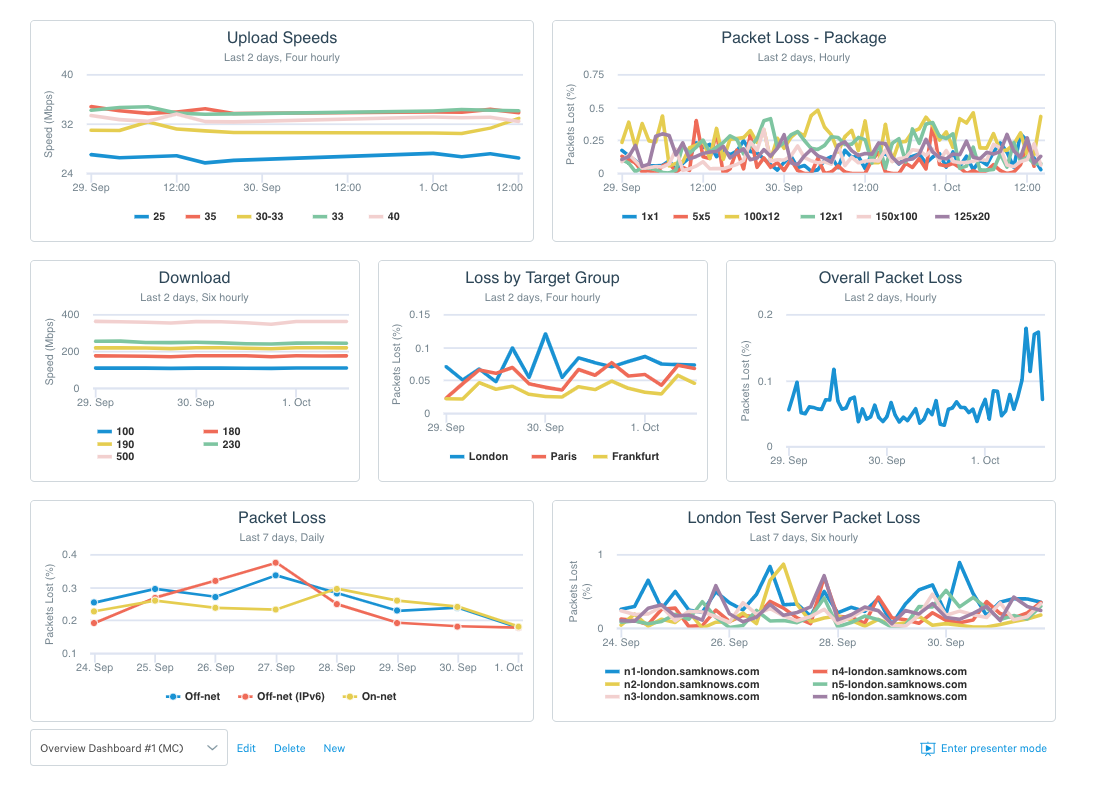
\includegraphics[width=15cm]{samknows.png}
\caption{Screenshot of SamKnows One dashboard}
\label{fig:samknows}
\end{figure}

\subsubsection{SMAQ}
SMAQ is a solution implemented by Sofrecom to generate reports and analysis based upon different broadband tests, this solution is used by the Orient Middle East and Africa Orange affiliates. 

\begin{figure}[H]
\centering
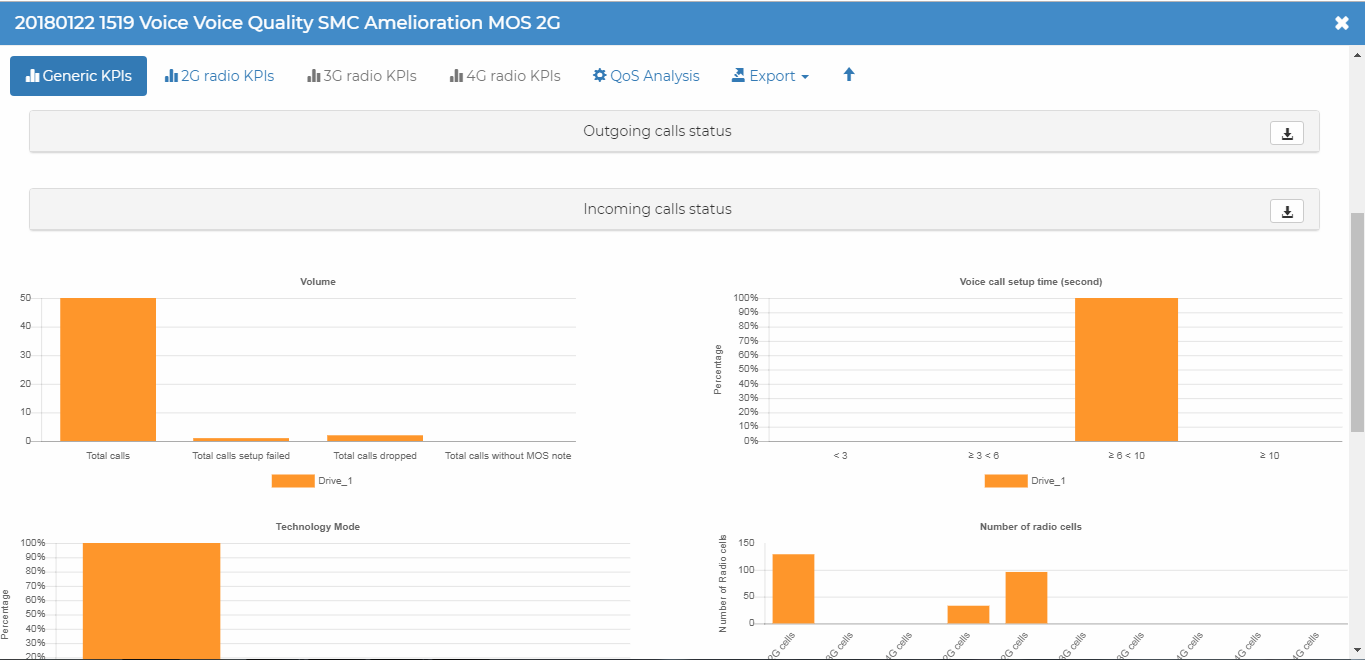
\includegraphics[width=15cm]{smaq.png}
\caption{Screenshot of SMAQ online dashboard}
\label{fig:smaq}
\end{figure}


\subsection{Critical of the state of the art}
The following table shows in detail the difference between the two mentioned solutions:
\begin{table}[H]
\centering
\begin{tabular}{|l|l|l|l|l|l|}
\hline
Solution                       & SamKnows One & SMAQ \\ \hline
Paying solution                      & YES         & NO \\ \hline
Analytics                 & YES         & YES \\ \hline
Custom dashboard & YES         & NO \\ \hline
Mapping data                 & YES         & NO  \\ \hline
Generate reports                    & YES         & YES  \\ \hline
Network monitoring (alerting)                    & YES         & YES \\ \hline
Users management              & YES          & NO \\ \hline
Devices management              & NO          & NO \\ \hline
Tests management              & NO          & NO \\ \hline
\end{tabular}
\caption{Comparison of state of the art}
\label{my-label}
\end{table}


Sofrecom Tunisia is looking for an open source solution for the issue in question so SamKnows One solution is not convenient for them, in the other hand SMAQ provides just the basic functionalities. The weak point in the mentioned solutions, they don’t give users the access to devices configuration. Network supervisors can’t customize tests to satisfy their specific needs.

\subsection{Proposed solution:}
The solution proposed by Sofrecom Tunisia is to design and develop a platform for broadband monitoring and supervision, “SMAQ Probes”, the solution should respond the following needs:

\begin{itemize}
\item	Online device management and task scheduling.
\item	Online test management.
\item	Online statistics and customized charts configuration.
\item	Online alerts configuration and customization.
\item	Online user management.
\end{itemize}

\section{Modeling language}
During the work on our solution we used UML “Unified Modeling Language” for describing and modeling the specifications of our project. UML is a flexible and versatile modeling language, also it is the most popular and widely used by the community. We are going to present some diagrams from UML that we find it useful during our work:

\begin{itemize}
\item	Use case diagram: it helps to structure the needs of users and the corresponding objectives of our system by identifying its users and their interactions.
\item	Sequence diagram: it is a time focus representation of objects and their interactions.
\item	Package diagram: it gives an overview of the application packages. It is a high abstraction that presents the application modularity.
\item	Class diagram: it gives a presentation of classes and interfaces of our system and relations between them.
\end{itemize}

\section{Software development methodology}
Before starting the project design and development, we should choose appropriate software development methodology to work with. The software development methodology helps to describe the different phases and the sequences of application development process.

During our project, we used agile kanban because it is a most convenient method to us. I am the only intern working on the project. Changes in the project can happen any time. We are continuously improving the flow of work. We are trying to limit work in progress and to maximize efficiency. Also, we focus on reducing the time it takes to take a project from start to finish.


\section{Conclusion}

In this chapter, we presented the general context of the project by presenting the host company Sofrecom Tunisia, the problem statement and the state of the art.

In the next chapter, we will model the requirements of our solution through use case diagrams.

\chapter{Requirements Analysis and Specification}

\section{Introduction}

The requirements analysis and specification phase is an essential step for the development of a new application. It allows presenting the application’s features in detail.

In this chapter, the first part will be devoted to identify the different actors of the application who are interacting with the system and to give the functional and nonfunctional requirements definitions. Subsequently, we will present the general system analysis using use case diagrams.

\section{Identification of the actors:}
An actor is an abstraction of a role of actual user who is in a perpetual interaction with the application. Following on, our system’s actor along with his role and granted permissions.

\subsection*{Internal actors}

\begin{itemize}
\item	Application administrator: the administrator is responsible of managing users and their permission, he has the permission to create, read, update, and delete users. Also, he has the permission to check all the other configurations like devices configuration and test configuration.
\item	Network supervisor: the network supervisor has the permission to read the different configurations without editing them. He has the right to supervise the quality of experience “QOS”.
\item	Network and broadband administrator: he has all the rights of the network supervisor, in addition, he has the permission to create, read, update, and delete broadband monitoring configurations.
\end{itemize}

\subsection*{External actors}

\begin{itemize}
\item	Probe: the probe is the entity able to get devices and tests configuration, and send the metrics to the server after running tests.
\end{itemize}

\section{Functional requirements}

Functional requirements refer to primary functions that each component of our solution must exhibit. It is a set of services which are:
\subsection*{For the web application}

\begin{itemize}
\item	The application should give the administrator the hand to manage users’ accounts.
\item	The application should give permitted users the possibility to customize their dashboards.
\item	The application should give permitted users the access to manage the network monitoring (alerting).
\item	The application should provide permitted users with the access to tests and devices configurations.
\item	The application should be able to process received metrics data in real-time.
\end{itemize}

\subsection*{For the hardware}

\begin{itemize}
\item	The boards should be able to receive and implement their configurations in real-time.
\item	The boards should be able to run tests according to the time scheduler and send results to the server.
\item	The boards should be able to send their current configuration (location, IP address, device identifier, jobs configuration).
\item	The boards should be able to keep the tests results if the server is not available.
\end{itemize}

\section{Non-functional requirements}
Non-functional requirements refer to several key features that are beyond the purpose of the solution, they specify criteria that judge the operation of a system, rather than specific behaviors in order to ensure the client’s satisfaction.
\paragraph{Extensibility}
~\\
The system must be open to some extension like for example adding new features if needed without radical modification in the code.
\paragraph{Performance}
~\\
The web application should be as efficient as possible with especially a good response time. Users should be able to receive the quality of experience (QOE) from the cloud server within a reasonable amount of time.
\paragraph{Re-usability}
~\\
The system shouldn’t be exclusive for our case and must be adaptive to other use cases.
\paragraph{Robustness}
~\\
The system must cope with errors during execution and should be able to reboot within a short time in case of failure.
\paragraph{Security}
~\\
The user’s personal information must be kept safe from others and only system administrator has permissions to access it. The broadband monitoring and supervision access must be permitted to the supervisors of the network in question.

\section{Requirements analysis}
On one hand, this section offers a better understanding of the mentioned requirements by declaring them in a semi-formal way. On the other hand, it emphasizes the interactions between the actor and our application. In contemplation of breaking down the complexity of these goals, we use the use case diagrams. 

\begin{figure}[H]
\centering
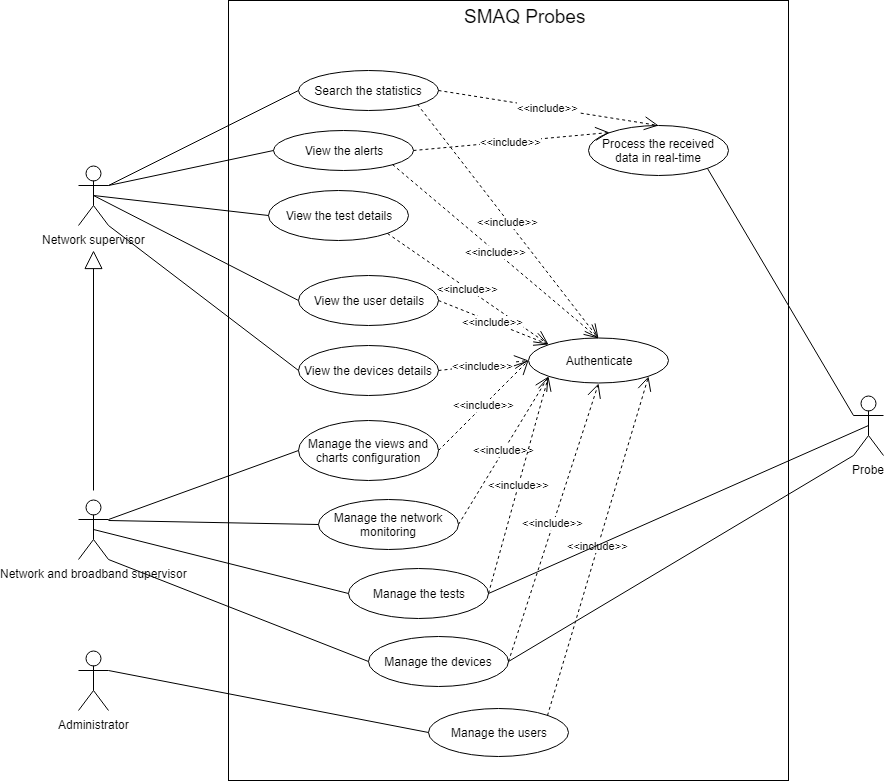
\includegraphics[width=15cm,height=16cm]{general-use-case-diagram.png}
\caption{General use case diagram}
\label{fig:usecasegeneral}
\end{figure}

As shown in the general use case diagram (fig.\ref{fig:usecasegeneral}), only the administrator can register all types of users. All the features of the application must go through authentication. The network and broadband supervisor is responsible for managing network monitoring, devices configuration, tests, and statistics configuration. Any configuration that concerns probes configuration will be sent to probes. Probes send their information and runs tests according to a job scheduler, then probes send tests results to the server, thus, our system process the received data in real-time. Finally our system is prepared to generate statistics and quality of service for the network supervisor.

\subsection{Manage devices}

\begin{figure}[H]
\centering
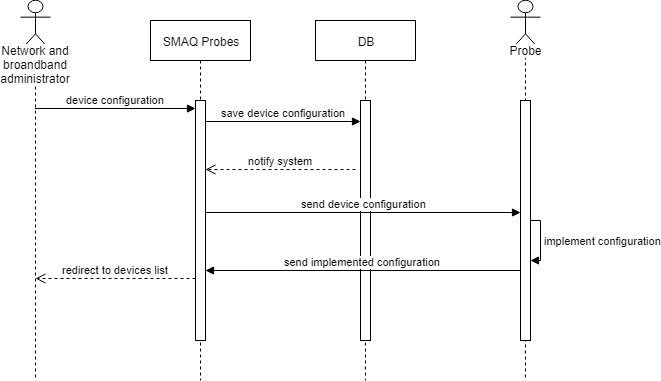
\includegraphics[width=15cm, height=13cm]{manage-device-sequece-diagram.png}
\caption{Devices management sequence diagram}
\label{fig:devicesequence}
\end{figure}

\begin{table}[H]
\centering
\begin{tabular}{|l|l|}
\hline
Title             & Device management                                                                                                                                                                                                                                                                                    \\ \hline
Author            & Ismail MEKNI                                                                                                                                                                                                                                                                             \\ \hline
Version           & 1.0                                                                                                                                                                                                                                                                                             \\ \hline
Objectives        & Allow users to manage connected devices configuration
 \\ \hline
Actors            & \begin{tabular}[c]{@{}l@{}}Network and broadband administrator – SMAQ Probes – \\Probe\end{tabular}                                                                                                                                                                                                                                                                                                                                                                                                                                                                                                                                                                                                                                                                                                          \\ \hline
Pre-conditions    & \begin{tabular}[c]{@{}l@{}}The user should authenticate as network and broadband\\ administrator.\\ The device should be connected.\end{tabular}                                                                                                                                                                  \\ \hline
Post-conditions   & \begin{tabular}[c]{@{}l@{}}New device configuration is persisted in the database.\\ New device configuration is implemented in the probe.\end{tabular}                                                                                                                                                                                                                                                                                                                                                                                                                             \\ \hline
Story             & \begin{tabular}[c]{@{}l@{}}1. The user enters device new configuration (status, \\IP address, client name, job scheduling).\\ 2. The user submits the changes.\end{tabular}                                                                                    \\ \hline
Alternative story & \begin{tabular}[c]{@{}l@{}}\end{tabular}                                                                                                                                                                            \\ \hline
Exceptional story & \begin{tabular}[c]{@{}l@{}}The device in question is not connected; the configuration’s\\ message will be suspended waiting the device to reconnect.\end{tabular} \\ \hline
\end{tabular}
\caption{Device management description}
\label{my-label}
\end{table}

As shown in the devices management sequence diagram (fig.\ref{fig:devicesequence}), the device management functionality is permitted to network and broadband administrators. User can access to the devices list. User can select a device to edit its configuration (IP address, location, registered client name, job scheduling), if user submits the new configuration, the configuration will be sent to the backend system to persist it to database. Also the configuration will be sent to the device in question, the probe, device, implements the changes. Finally, the probe sends back the implemented configurations to the system as a confirmation.

\subsection{Manage tests}

\begin{figure}[H]
\centering
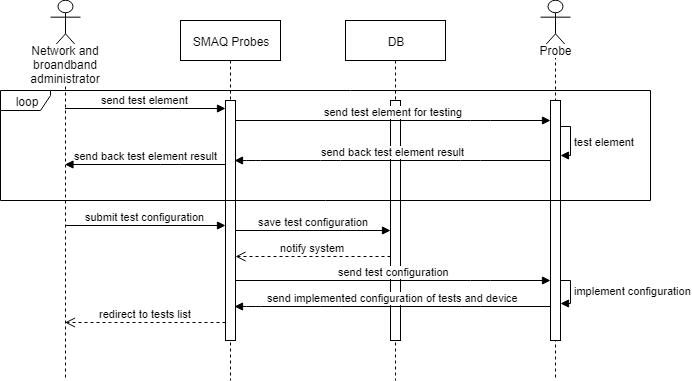
\includegraphics[width=15cm, height=13cm]{tests-management-sequence-diagram.png}
\caption{Tests management sequence diagram}
\label{fig:testsequence}
\end{figure}

\begin{table}[H]
\centering
\begin{tabular}{|l|l|}
\hline
Title             & Tests management                                                                                                                                                                                                                                                                                    \\ \hline
Author            & Ismail MEKNI                                                                                                                                                                                                                                                                             \\ \hline
Version           & 1.0                                                                                                                                                                                                                                                                                             \\ \hline
Objectives        & Allow users to manage tests configuration.
 \\ \hline
Actors            & \begin{tabular}[c]{@{}l@{}}Network and broadband administrator – SMAQ Probes – \\Probe\end{tabular}
\\ \hline
Pre-conditions    & \begin{tabular}[c]{@{}l@{}}The user should authenticate as network and broadband \\administrator.\\ At least one device should be connected.\end{tabular}                                                                                                                                                                  \\ \hline
Post-conditions   & \begin{tabular}[c]{@{}l@{}}New tests configuration is persisted in the database.\\ New tests are running on the probes.\end{tabular}                                                                                                                                                                                                                                                                                                                                                                                                                             \\ \hline
Story             & \begin{tabular}[c]{@{}l@{}}1. The user tests each element directly on the device.\\ 2. The user submits the test configuration with all elements.\end{tabular}                                                                                    \\ \hline
Alternative story & \begin{tabular}[c]{@{}l@{}}\end{tabular}                                                                                                                                                                            \\ \hline
Exceptional story & \begin{tabular}[c]{@{}l@{}}There is no connected device, so user can’t test elements,\\ the operation with be suspended until at least one device\\ reconnect.\end{tabular} \\ \hline
\end{tabular}
\caption{Test management description}
\label{my-label}
\end{table}

As shown above in the diagram (fig.\ref{fig:testsequence}), the access to the test configuration is granted to users with network and broadband administrator role. To edit test configuration, user should enter test elements, each element must be tested directly on the probe, device, and then test’s element result will be sent back to the user. After creating and testing all the elements, a new test configuration will be sent to the backend system. The configuration is persisted to database. The new test configuration is sent to the probes, all the probes implement the new test configuration. Finally a signal messages is sent from all the probes holding the current configurations.

\subsection{Manage network monitoring}

\begin{figure}[H]
\centering
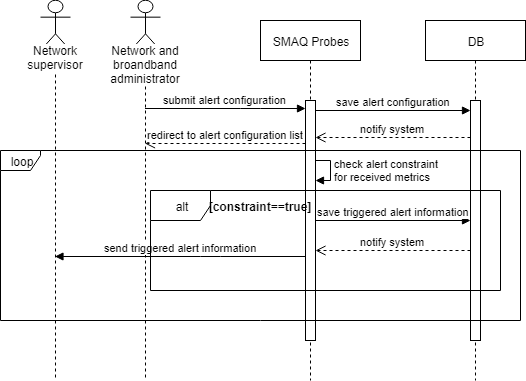
\includegraphics[width=15cm, height=14cm]{network-monitoring-management-sequence-diagram.png}
\caption{Network monitoring management sequence diagram}
\label{fig:monitoringsequence}
\end{figure}

\begin{table}[H]
\centering
\begin{tabular}{|l|l|}
\hline
Title             & Network monitoring management
\\ \hline
Author            & Ismail MEKNI                                                                                                                                                                                                                                                                             \\ \hline
Version           & 1.0                                                                                                                                                                                                                                                                                             \\ \hline
Objectives        & \begin{tabular}[c]{@{}l@{}} Allow users to manage network monitoring configuration,\\ alerting system.\end{tabular}
 \\ \hline
Actors            & \begin{tabular}[c]{@{}l@{}}Network and broadband administrator – Network supervisor\\ – SMAQ Probes\end{tabular}
\\ \hline
Pre-conditions    & \begin{tabular}[c]{@{}l@{}}The user should authenticate as network and broadband \\administrator to access the network monitoring management.\\ To view triggered alerts, the user should authenticate as a\\ network supervisor.\end{tabular}                                                                                                                                                                  \\ \hline
Post-conditions   & \begin{tabular}[c]{@{}l@{}}New alert configuration is persisted in the database.\\ Alert listener is running on the received metrics.\end{tabular}                                                                                                                                                                                                                                                                                                                                                                                                                             \\ \hline
Story             & \begin{tabular}[c]{@{}l@{}}1. The user send alert configuration containing the constraint.\\ 2. The network supervisor can view alerts if triggered.\end{tabular}                                                                                    \\ \hline
Alternative story & \begin{tabular}[c]{@{}l@{}}\end{tabular}                                                                                                                                                                            \\ \hline
Exceptional story & \begin{tabular}[c]{@{}l@{}}\end{tabular} \\ \hline
\end{tabular}
\caption{Network monitoring management description}
\label{my-label}
\end{table}

As shown in the diagram (fig.\ref{fig:monitoringsequence}), the user authenticates with network and broadband administrator. This feature aims to configure customized alerts. User creates alerts with a specific constraint. This configuration will be persisted to database. An alert checker will be run for every received metrics data, if the constraint is satisfied an alert with full description will be triggered. The triggered alerts are persisted to database so network supervisors can check them.

\subsection{Manage statistics and charts configuration}

\begin{figure}[H]
\centering
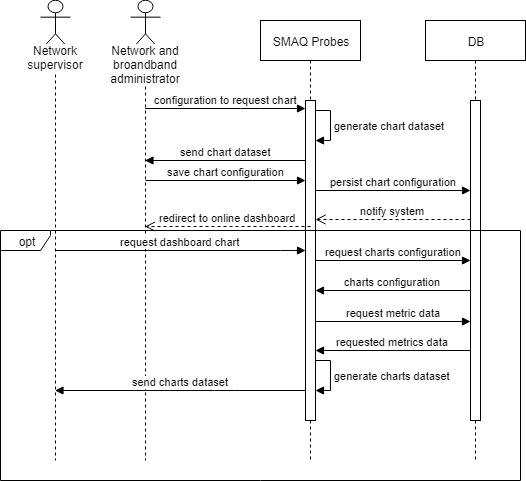
\includegraphics[width=15cm, height=14cm]{charts-management-sequence-diagram.png}
\caption{Charts management sequence diagram}
\label{fig:chartssequence}
\end{figure}

\begin{table}[H]
\centering
\begin{tabular}{|l|l|}
\hline
Title             & Charts and statistics management
\\ \hline
Author            & Ismail MEKNI                                                                                                                                                                                                                                                                             \\ \hline
Version           & 1.0                                                                                                                                                                                                                                                                                             \\ \hline
Objectives        & Allow users to manage charts configuration.
 \\ \hline
Actors            & \begin{tabular}[c]{@{}l@{}}Network and broadband administrator – Network supervisor\\ – SMAQ Probes\end{tabular}
\\ \hline
Pre-conditions    & \begin{tabular}[c]{@{}l@{}}The user should authenticate as network and broadband \\administrator to access charts and statistics management.\\ To view dashboard, the user should authenticate as a \\network supervisor.\end{tabular}                                                                                                                                                                  \\ \hline
Post-conditions   & \begin{tabular}[c]{@{}l@{}}New chart configuration is persisted in the database.\\ New chart is added to dashboard.\end{tabular}                                                                                                                                                                                                                                                                                                                                                                                                                             \\ \hline
Story             & \begin{tabular}[c]{@{}l@{}}1. The user send chart configuration, system generates chart \\dataset.\\ 2. Chart displayed to user.\\ 3. User submit chart configuration.\end{tabular}                                                                                    \\ \hline
Alternative story & \begin{tabular}[c]{@{}l@{}}\end{tabular}                                                                                                                                                                            \\ \hline
Exceptional story & \begin{tabular}[c]{@{}l@{}}\end{tabular} \\ \hline
\end{tabular}
\caption{Charts management description}
\label{my-label}
\end{table}

As we can see in the above sequence diagram (fig.\ref{fig:chartssequence}), to access to charts and statistics configuration, users should have network and broadband administrator privileges. User enters the chart parameters; our system generates the chart in question. User submits this configuration to be persisted and added to dashboard. Thus, users with network supervisor permission can see the configured charts on the dashboard. This feature aims to allow users to create customized charts and views.

\subsection{Manage users}

\begin{figure}[H]
\centering
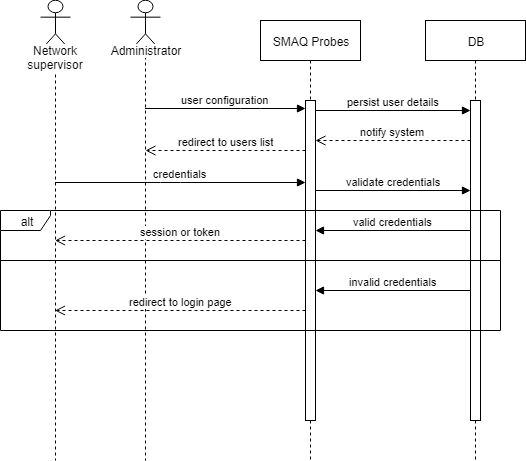
\includegraphics[width=15cm, height=14cm]{users-management-sequence-diagram.png}
\caption{Users’ management sequence diagram}
\label{fig:userssequence}
\end{figure}

\begin{table}[H]
\centering
\begin{tabular}{|l|l|}
\hline
Title             & Users management
\\ \hline
Author            & Ismail MEKNI                                                                                                                                                                                                                                                                             \\ \hline
Version           & 1.0                                                                                                                                                                                                                                                                                             \\ \hline
Objectives        & \begin{tabular}[c]{@{}l@{}}Allow administrator to manage users’ configuration and \\details.\end{tabular}
 \\ \hline
Actors            & \begin{tabular}[c]{@{}l@{}}Administrator – Network supervisor – SMAQ Probes\end{tabular}
\\ \hline
Pre-conditions    & \begin{tabular}[c]{@{}l@{}}The user should authenticate as application administrator to \\access the users’ management.\end{tabular}                                                                                                                                                                  \\ \hline
Post-conditions   & \begin{tabular}[c]{@{}l@{}}User credential is persisted to database.\\User can authenticate.\end{tabular}                                                                                                                                                                                                                                                                                                                                                                                                                             \\ \hline
Story             & \begin{tabular}[c]{@{}l@{}}1. The administrator submit user configuration.\\ 2. The user submits his credentials.\end{tabular}                                                                                   
 \\ \hline
Alternative story & \begin{tabular}[c]{@{}l@{}}\end{tabular}                                                                                                                                                                            \\ \hline
Exceptional story & \begin{tabular}[c]{@{}l@{}}If the user enters invalid credentials, he will be prompted to \\try to login again.\end{tabular} \\ \hline
\end{tabular}
\caption{Users management description}
\label{my-label}
\end{table}

As shown in the users' management sequence diagram (fig.\ref{fig:userssequence}), the users’ management feature is only allowed to the application administrator. The administrator enters the credentials of each user. Thus, user is now registered to the application and he can access to the application features according to his privileges. To sign in to the application, the user enters his credentials, generally a username and a password, if the credentials are valid, he will be redirected to the dashboard, and else he will be prompted to login again. 

\section{Conclusion}

Throughout this chapter, we specified and analyzed the requirements that solution should deliver to users, and we presented the main scenarios and the use cases that it should offer.

The next chapter aims to go a step further in the process of developing the application via presenting the design of the different components of our system.


\chapter{Design of the Physical and Logical Architectures}

\section{Introduction}
In order to reach the appropriate result as described in the specifications, we need to clarify the project’s main architecture as well as the architecture of its components. This chapter will focuses on designing a suitable structure for the smart parking system. This step is considered as the most crucial of the process because it prepares the ground for the implementation phase.

\section{Physical architecture}
The architecture presented in (fig.\ref{fig:physicalarchitecture}) is the physical architecture of our system. 
It represents the physical layout of our system and its components in a global diagram and it refers to some representations of the structure or organization of the physical elements that build the system.

\begin{figure}[H]
\centering
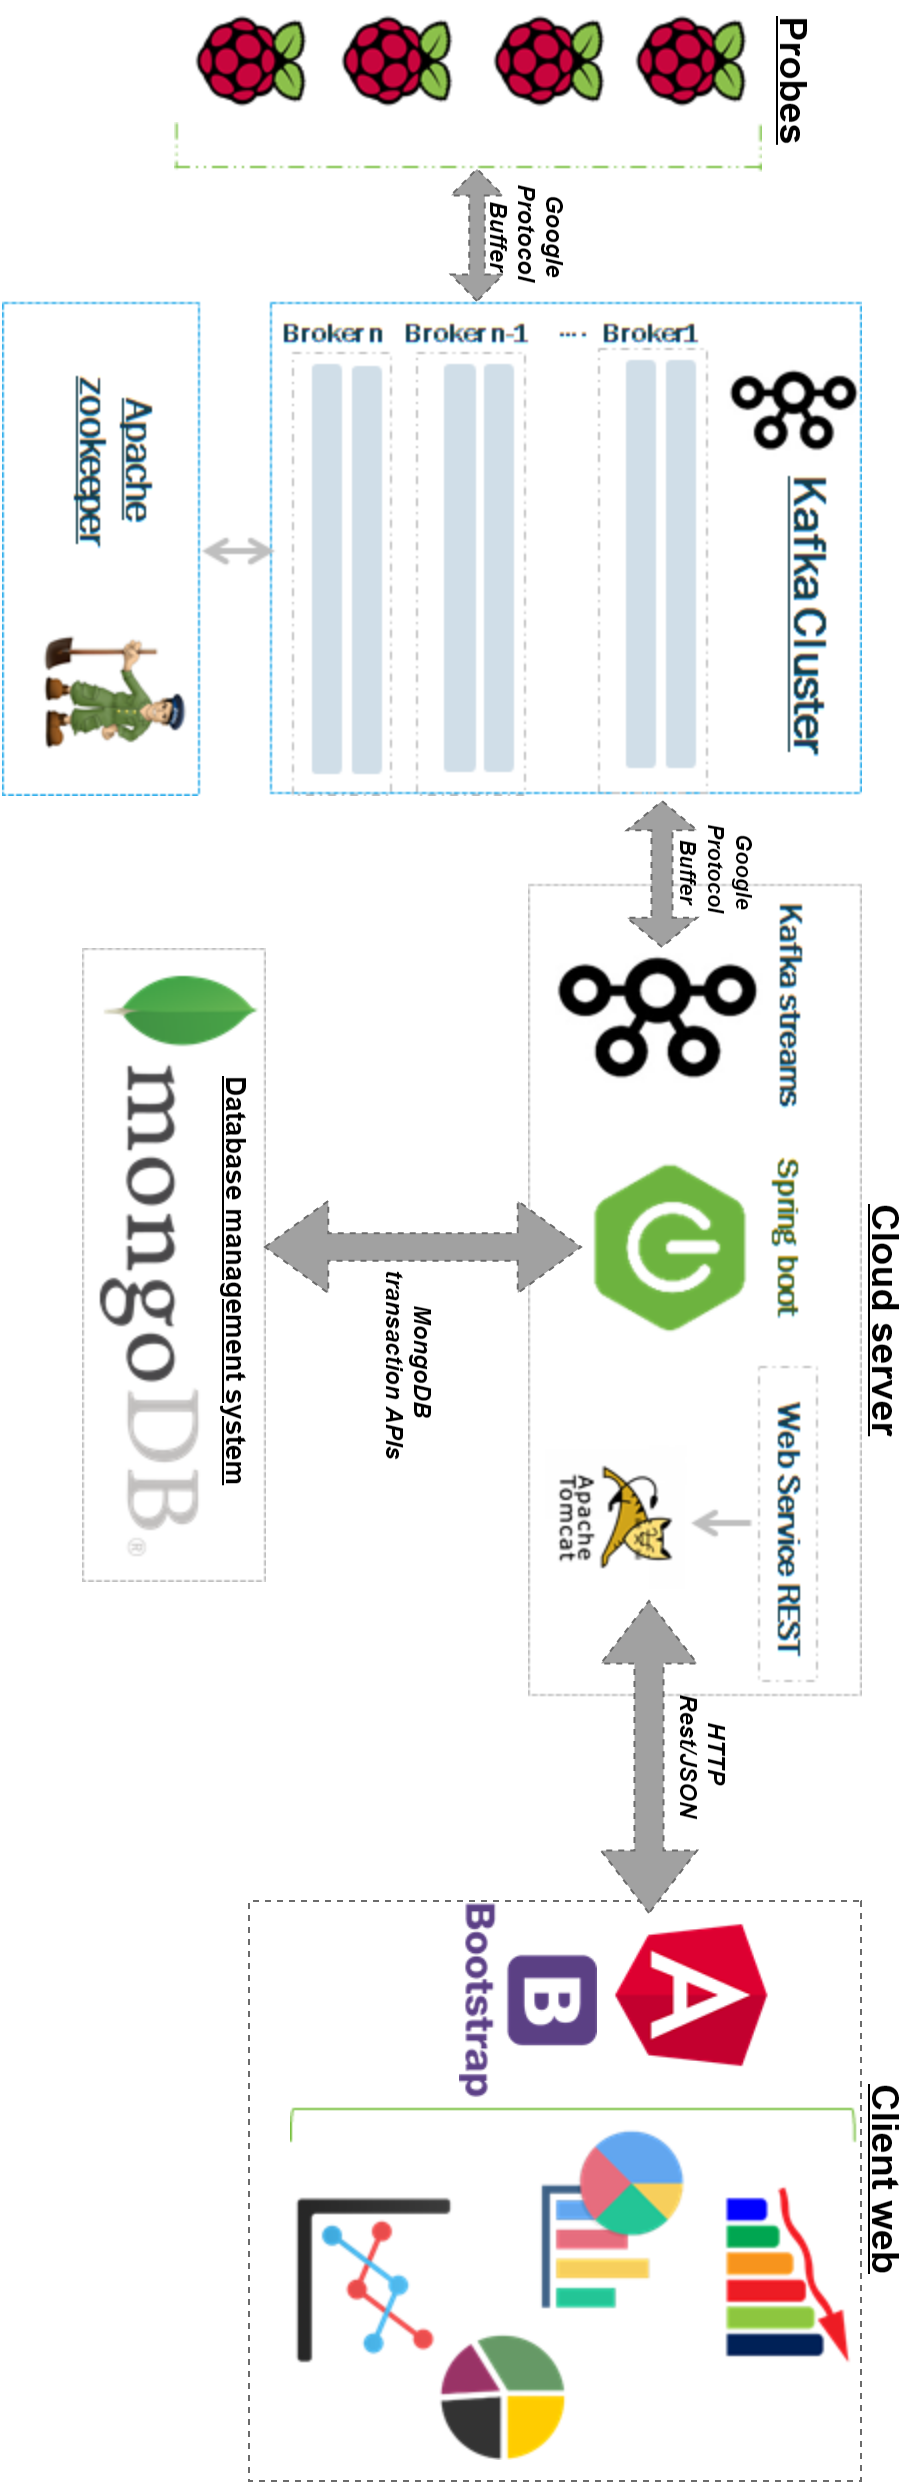
\includegraphics[height=25cm]{physicalarchitecture.png}
\caption{Physical Architecture of SMAQ Probes solution}
\label{fig:physicalarchitecture}
\end{figure}

This architecture describes the main components of the system and how they interact in order to achieve the objectives mentioned in the previous chapter.

The system is composed mainly from the following parts: the probes (Raspberry Pi boards), the user interface (web browser) and the cloud server including Kafka cluster, the database management system and our web application.

The probes represent the entity that executes the scheduled tests and sends the metrics to Kafka cluster through the Google protocol buffer.

The client web part represents the part with which the final users interacts and they are essentially: the Web platform accessible by the application users, application administrator, network supervisors and network and broadband administrators.

The third part, the cloud server, is where the application will be hosted, this part is responsible for receiving and processing data coming from Kafka cluster, also it is responsible for data analysis and configurations persistent to our database.

\section{Logical architecture}
\subsection{Conceptual model}
The (fig.\ref{fig:logicalarchitecture}) shows the logical architecture of the system.

\begin{figure}[H]
\centering
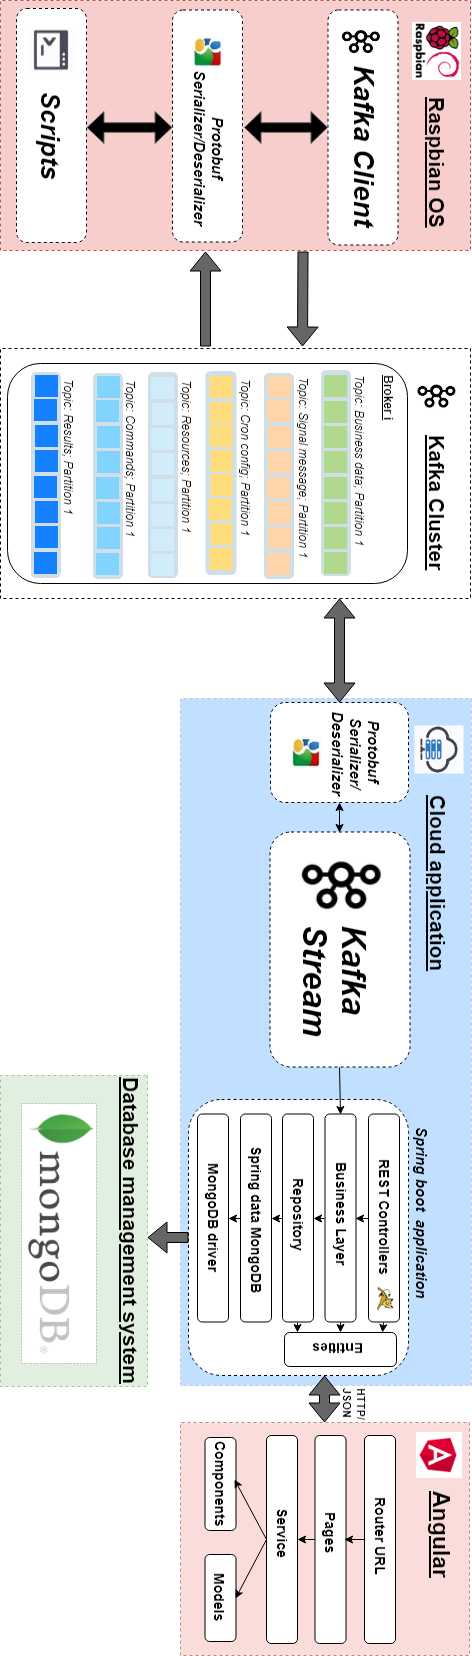
\includegraphics[height=25cm]{logicalarchitecture.png}
\caption{Logical architecture}
\label{fig:logicalarchitecture}
\end{figure}

According to the figure of the logical architecture, the system is composed from three major parts:
\begin{itemize}
\item	Probes: this parts represents widespread devices, these devices are the entities that handles tests. There are several scripts responsible for running the tests with efficient schedules. All the messages are serialized with Google Protocol Buffer. There is a Kafka client responsible for publishing and receiving messages\cite{RDKAFKA}.
\item	Cloud server: this server is the entity that holds the application logic. It holds within him a Google Protocol Buffer converter. Kafka stream is the layer that process the received data in real-time with high performance\cite{KAFKASTREAM}. Spring Boot application is a three tiers web application, it is responsible for managing the features of our system including metrics analytics.
\item	Angular: this entity is the frontend application accessible to users across the Web\cite{ANGULAR}.
\end{itemize}

The connection between the web application and the user interface is guaranteed through HTTP protocol and REST web services.

Kafka cluster is playing the role of a middleware between the probes and the backend server.

Finally we have our database, we have chosen MongDB as a database management system for performance reasons, and it is accessible only through the three tiers web application.


\subsection{Modular decomposition}
\subsubsection{Class diagram of entities}
The (fig.\ref{fig:generalclassdiagram}) shows the class diagram of our system, this diagram summarizes relationships between our entities in the database.
This class diagram is efficient in the case of MongoDB database management system. MongoDB is an oriented document database management system.
\begin{figure}[H]
\centering
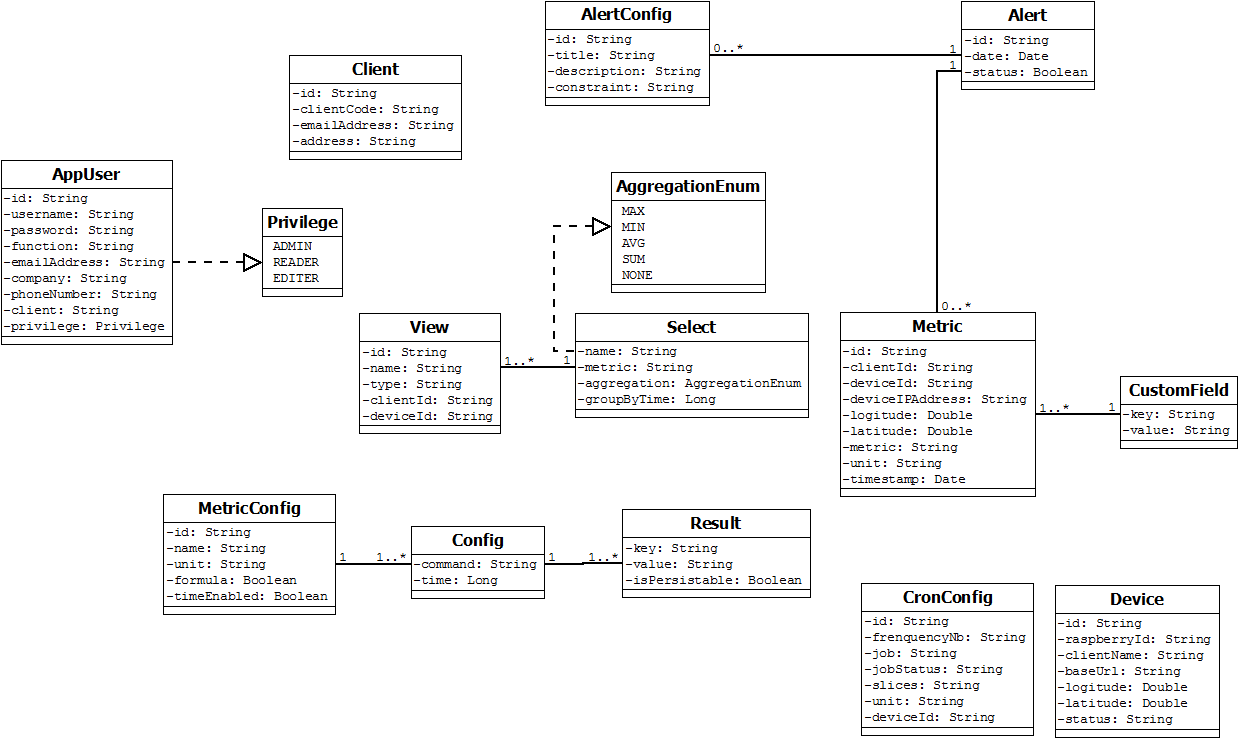
\includegraphics[height=25cm]{generalclassdiagram.png}
\caption{Database entities class diagram}
\label{fig:generalclassdiagram}
\end{figure}

\subsubsection{Package diagram}
The package diagram is a static view that serves to globally describe the different components of the application. The (fig.\ref{fig:packagediagram}) presents the package diagram of our solution to have an overview its different elements.
\begin{figure}[H]
\centering
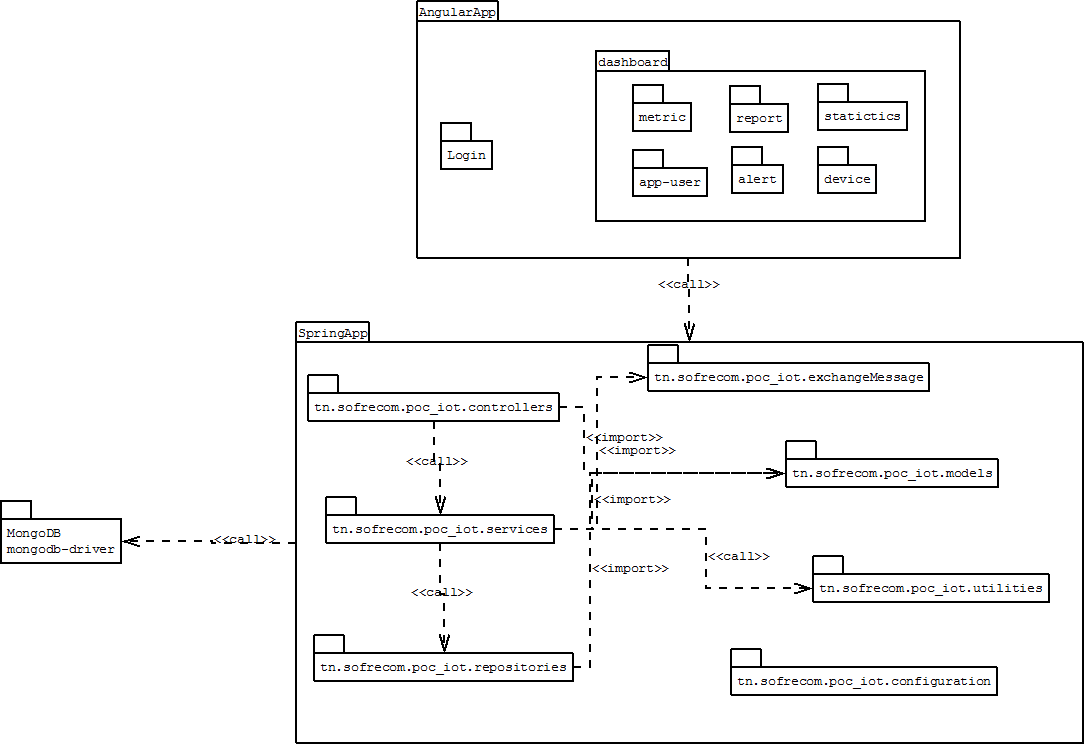
\includegraphics[width=15cm]{packagediagram.png}
\caption{Package diagram of the backend application}
\label{fig:packagediagram}
\end{figure}

\subsubsection{Devices management module}
This module describes devices management process. This module is about 	editing, deleting, and checking available devices. There is no meaning of creating device because the device information will be sent by the device if it is connected.

The following class diagram (fig.\ref{fig:deviceclassdiagram}) presents the involved classes and components that build the module.
\begin{figure}[H]
\centering
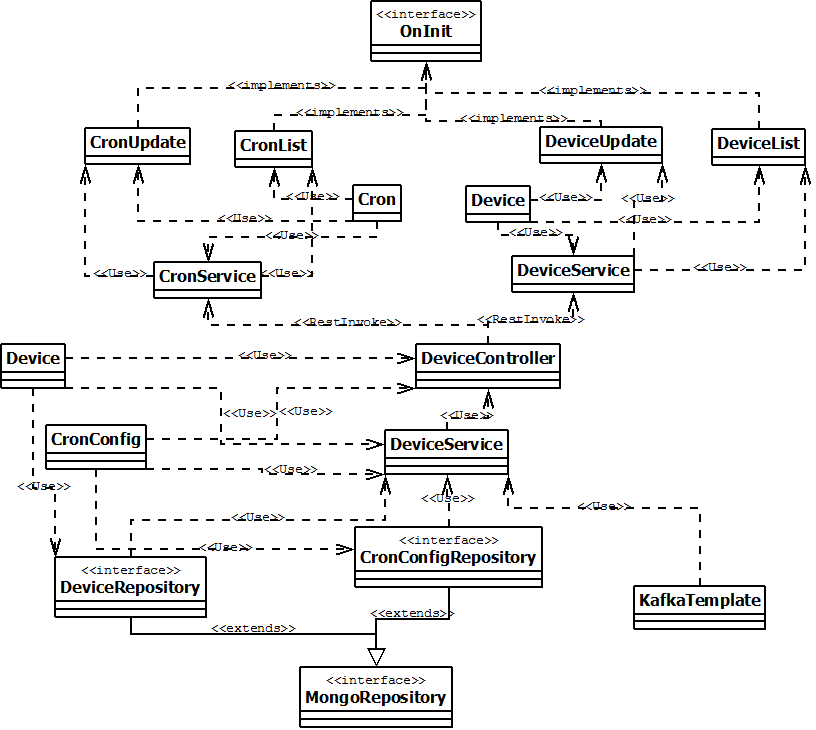
\includegraphics[width=15cm]{deviceclassdiagram.png}
\caption{Package diagram of the backend application}
\label{fig:deviceclassdiagram}
\end{figure}

Then, we have the sequence diagram that describes the interaction between the module components; this diagram presents the update device operation:

\begin{figure}[H]
\centering
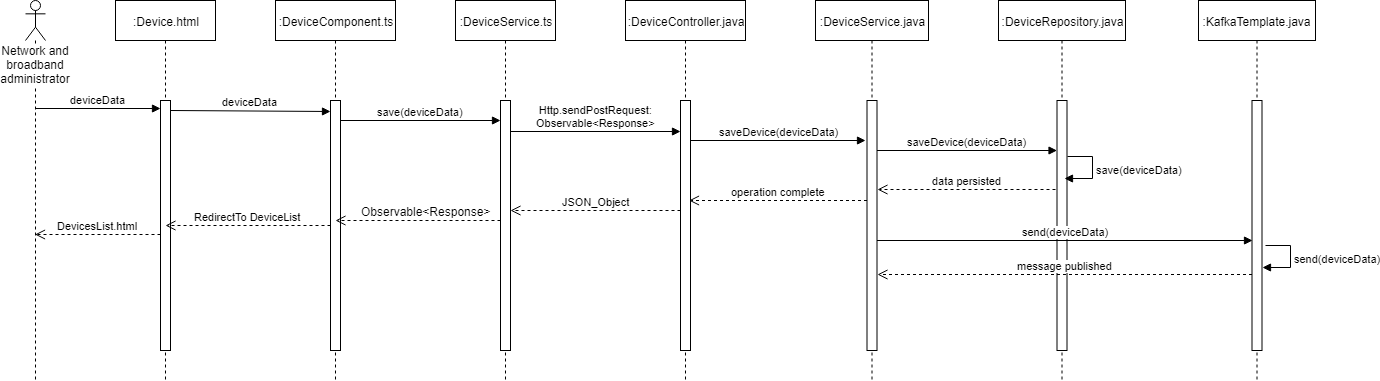
\includegraphics[width=17cm,height=10cm]{devicesequencediagram.png}
\caption{Sequence diagram of device updating operation}
\label{fig:devicesequencediagram}
\end{figure}

The diagram below is the sequence diagram for the update Cron operation. Cron is a job already running on the probe according to a specific schedule.

\begin{figure}[H]
\centering
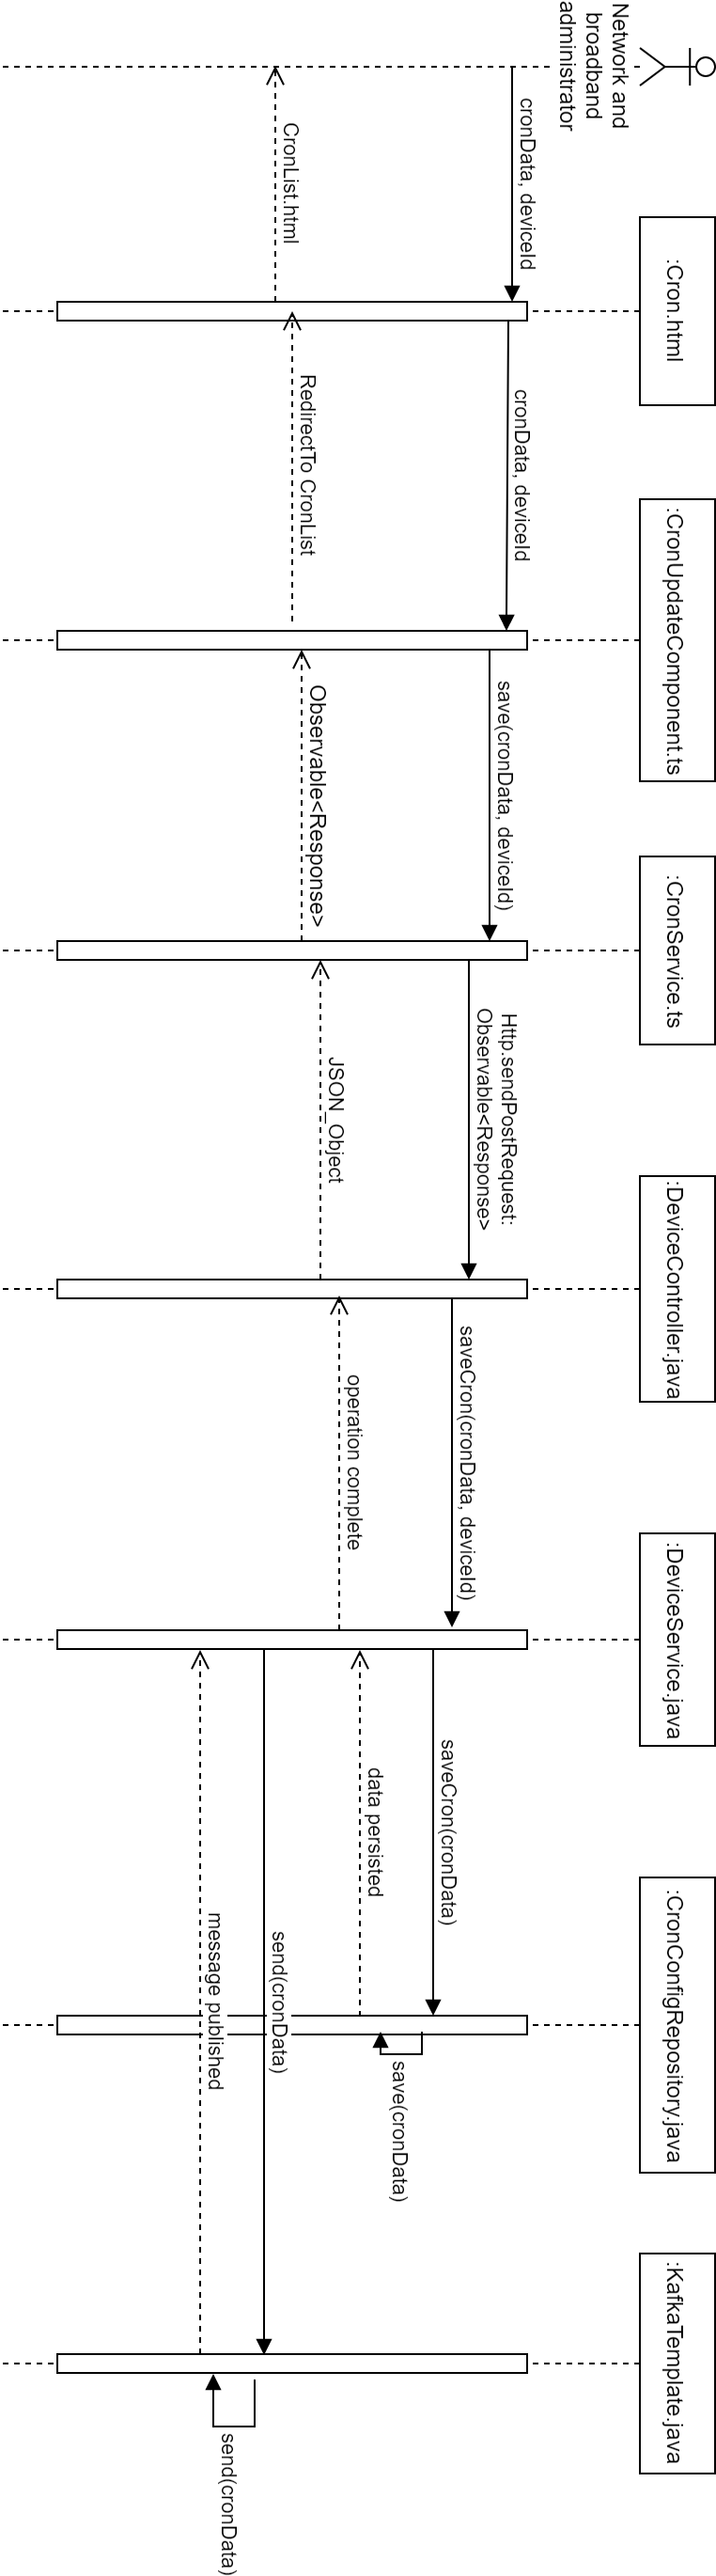
\includegraphics[width=17cm,height=10cm]{cronsequencediagram.png}
\caption{Sequence diagram of Cron updating operation}
\label{fig:cronsequencediagram}
\end{figure}

The device configuration consists of the device general information (IP address, device ID, location…) and the jobs running on the device in question. First, the user fills the form of device information, after, he submits this information. Using REST web services we deliver the new configuration from frontend application to backend side. Finally, the backend save the new configuration to our database and send it to the device in question in order to consider the new changes.

For Cron configuration, we follow the same process; the user submits the new configuration, after, this configuration will be sent to backend in JSON objects forma. Finally, our backend application implements the changes in the database and the device.


\subsubsection{Metrics and tests management module}
This module describes tests management process. This module is about creating, editing, deleting, and checking available devices.
The following class diagram (fig.\ref{fig:metricclassdiagram}) presents the involved classes and components that build our module.

\begin{figure}[H]
\centering
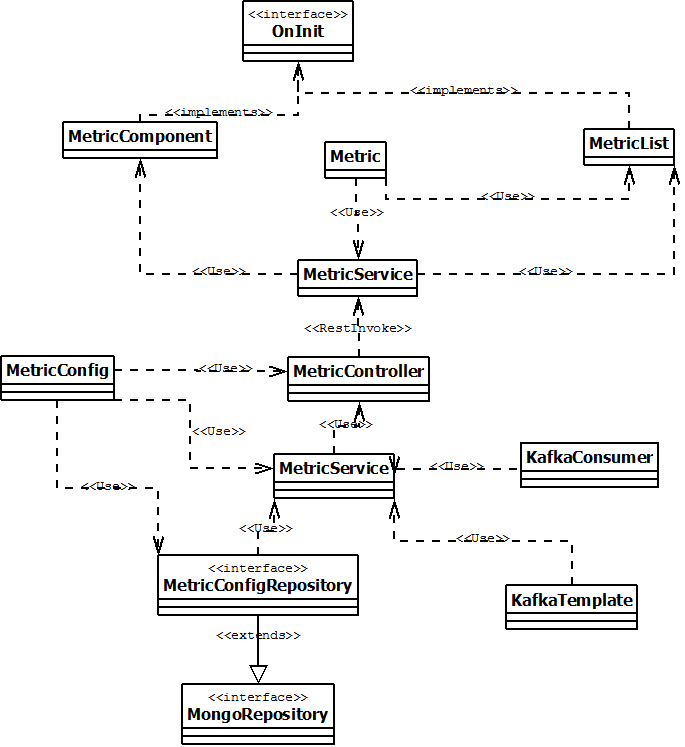
\includegraphics[width=15cm]{metricclassdiagram.png}
\caption{Class diagram of the tests and metrics management module}
\label{fig:metricclassdiagram}
\end{figure}

Then, we have the sequence diagram that describes the interaction between the module components; this diagram presents the creation and updating tests operations:

\begin{figure}[H]
\centering
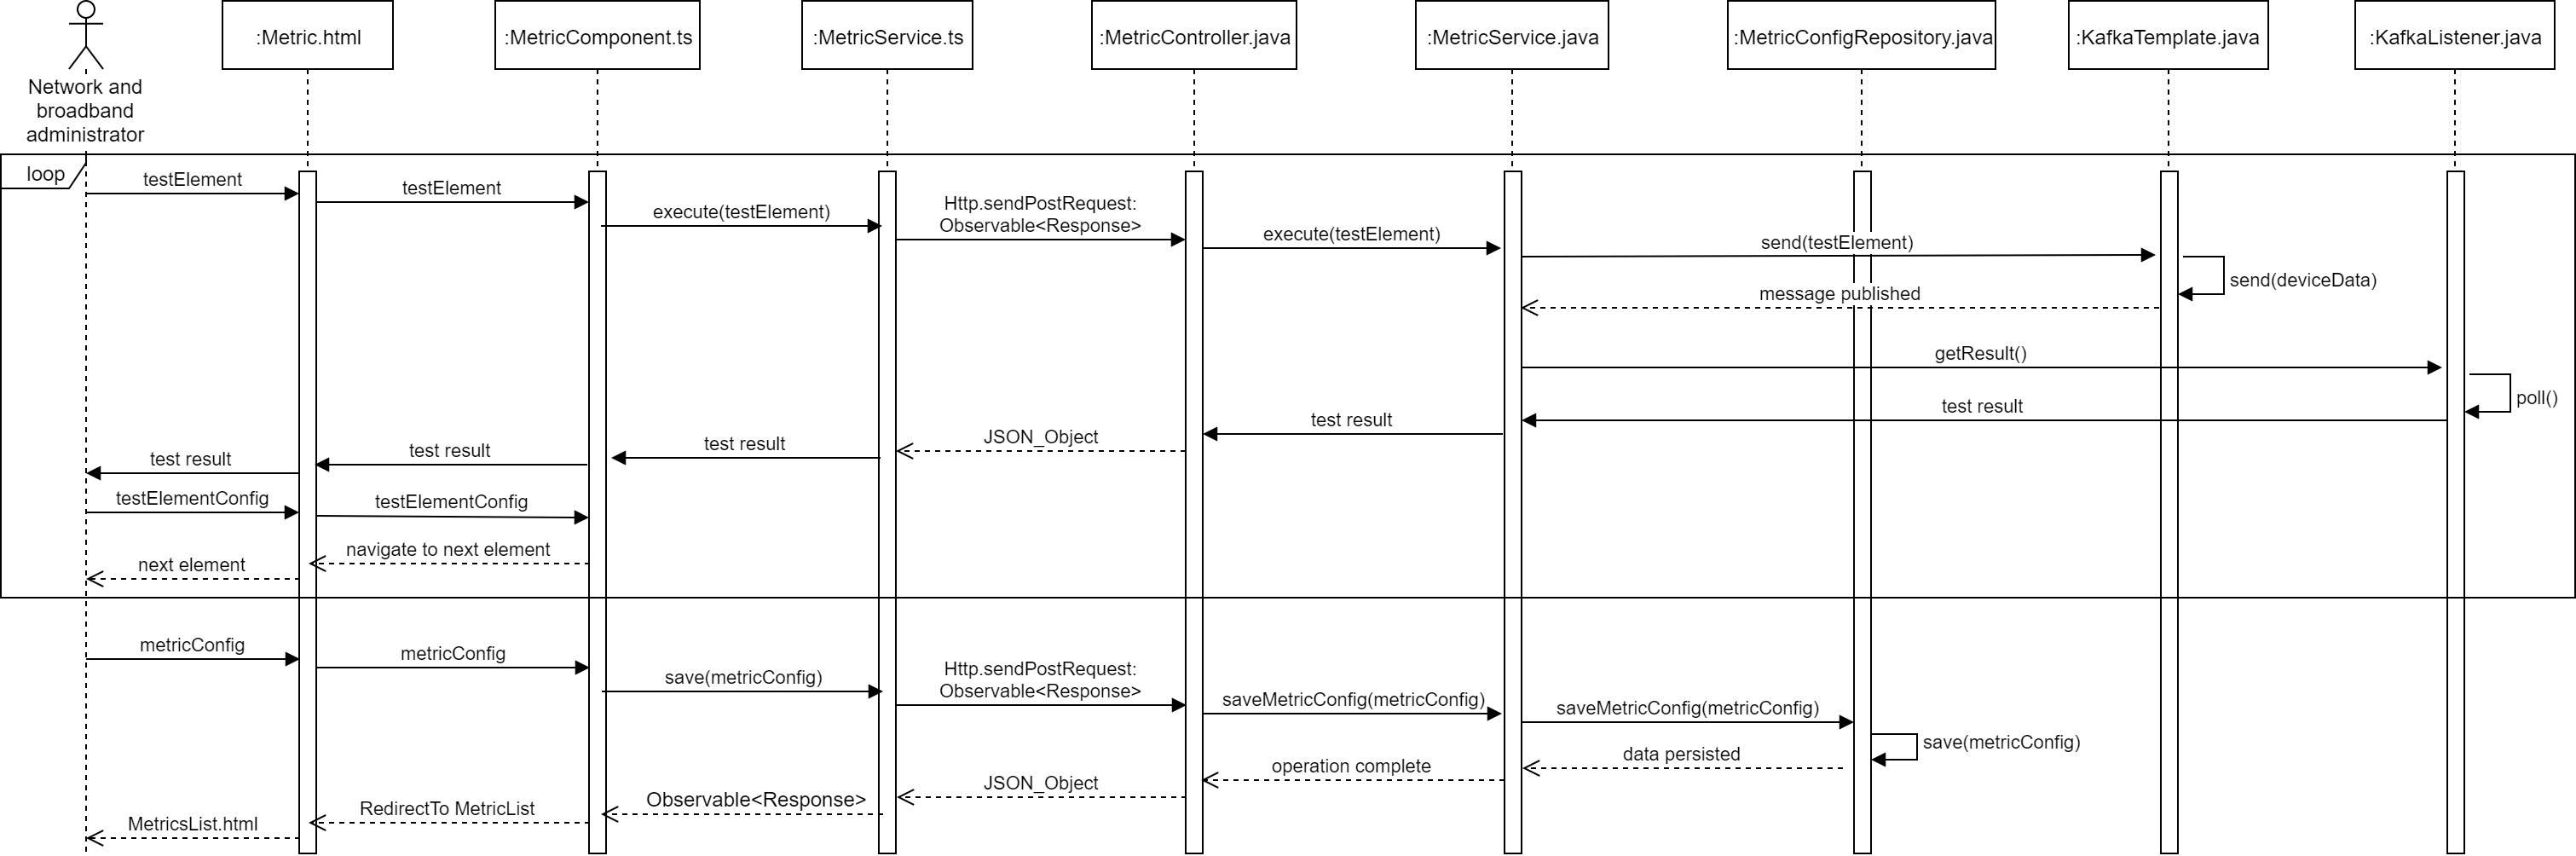
\includegraphics[width=17cm,height=10cm]{metricsequencediagram.png}
\caption{Sequence diagram of metrics and tests creation and updating operation}
\label{fig:metricsequencediagram}
\end{figure}

The metrics and tests configuration consists of the describing the general test information (test name, test unit, schedules) and the test elements configuration. A test element is a command line or even a script. To achieve better performance, each test element will be tested directly on the Raspberry board going through the frontend application to the backend application to reach our Kafka cluster, the element will be tested and the results will be sent back to Kafka, finally the results data will takes back the same path to reach the user interface. The user configures the element with its results. To finish, the user submits the entire test’s configuration to the web application.

We must note that the updating and creation operations are the same because we are using MongoDB as a database, if the object is already in the database, MongoDB will edit it, and else the object will be created.



\subsubsection{Network monitoring management module}
This module describes network monitoring management process. This module is about creating, editing, deleting, and checking available alerts information and constraints.

The following class diagram (fig.\ref{fig:alertclassdiagram}) presents the involved classes and components that build network monitoring module.

\begin{figure}[H]
\centering
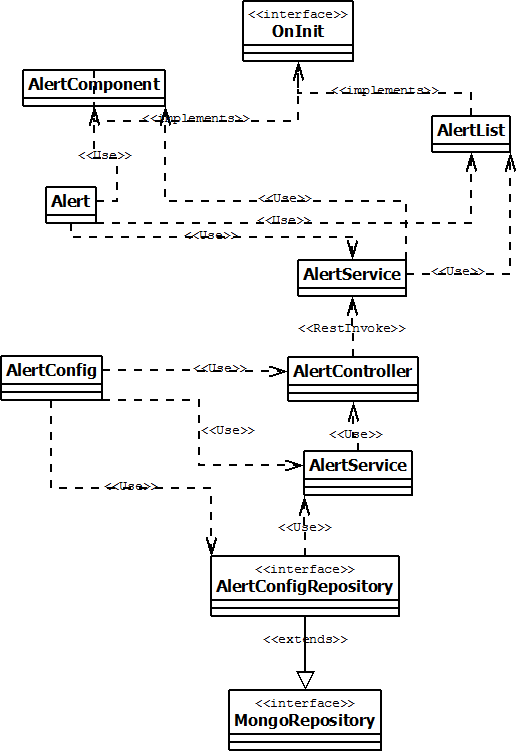
\includegraphics[width=15cm]{alertclassdiagram.png}
\caption{Class diagram of the network monitoring management module}
\label{fig:alertclassdiagram}
\end{figure}

Then, we have the sequence diagram that describes the interaction between the module components; this diagram presents the creation and updating alerts operations:

\begin{figure}[H]
\centering
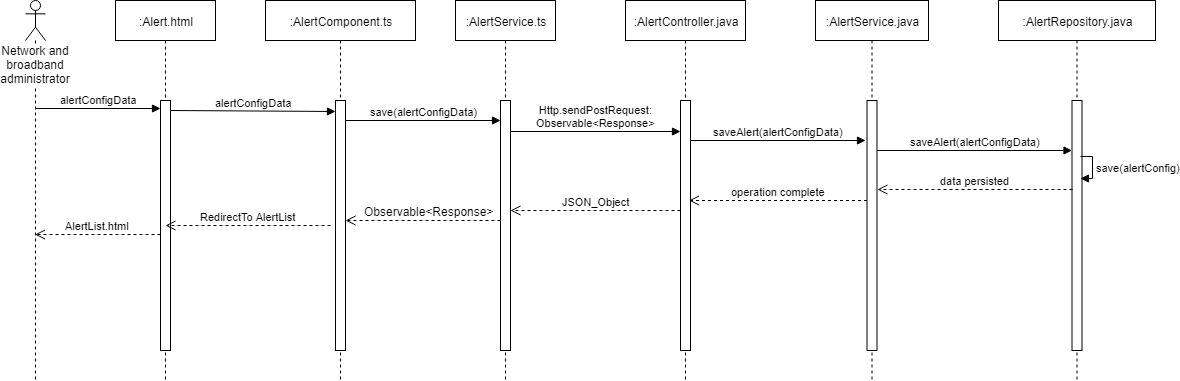
\includegraphics[width=17cm,height=10cm]{alertsequencediagram.png}
\caption{Sequence diagram of alerts creation and updating operation}
\label{fig:alertsequencediagram}
\end{figure}

The network monitoring configuration consists of creating customized alerts to help network supervisors. The network and broadband administrator fill the form that contains alert information (alert title, alert description, involved test, alert constraint) through the graphic user interface. The alert constraint is a logic expression that defines when the alert will be triggered. The configuration is sent from the frontend to backend with REST web services. The web application saves the alert configuration. The other details about the network monitoring concerning alert triggering and supervision will be explained and clarified in a separate part. 




\subsubsection{Statistics and charts management module}
This module describes statistics and charts management process. This module is about 	editing, deleting, and checking available charts and views. 

The following class diagram (fig.\ref{fig:viewclassdiagram}) presents the involved classes and components that build the module.

\begin{figure}[H]
\centering
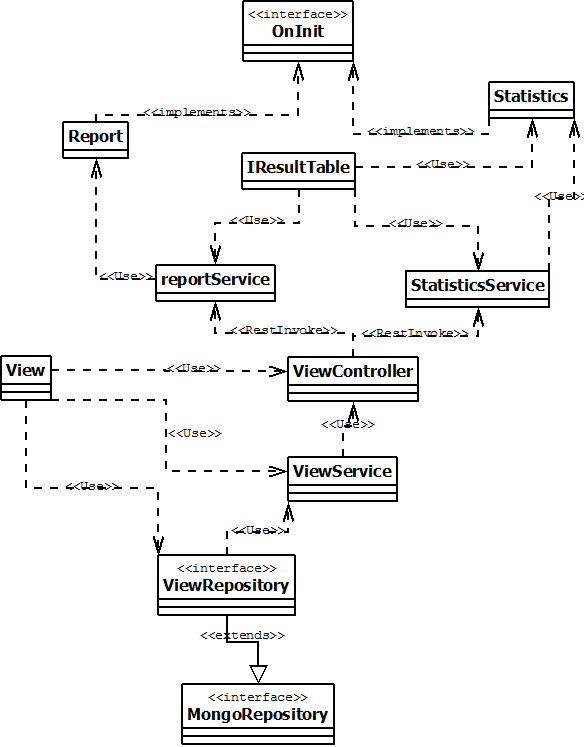
\includegraphics[width=15cm]{viewclassdiagram.png}
\caption{Class diagram of the statistics and charts management module}
\label{fig:viewclassdiagram}
\end{figure}

Then, we have the sequence diagram that describes the interaction between the module components; this diagram presents the creation views operation:

\begin{figure}[H]
\centering
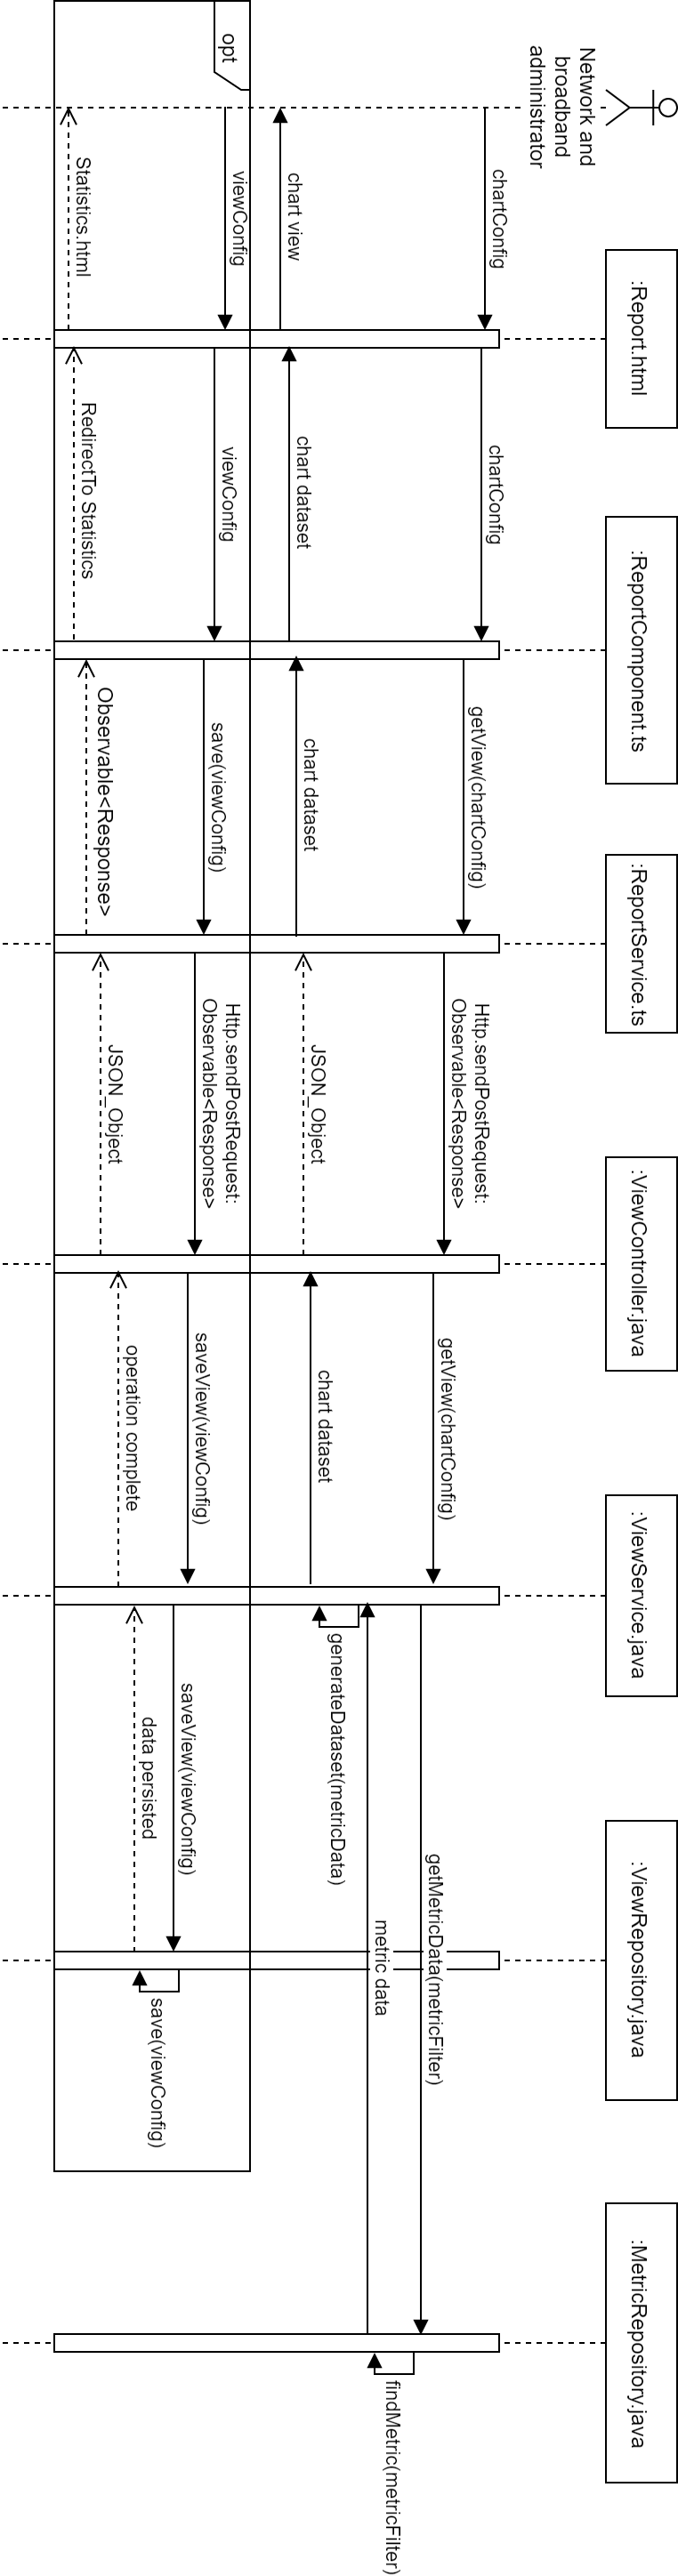
\includegraphics[width=17cm,height=10cm]{viewsequencediagram.png}
\caption{Sequence diagram of views creation operation}
\label{fig:viewsequencediagram}
\end{figure}

The diagram below is the sequence diagram for dashboard generation operation. 

\begin{figure}[H]
\centering
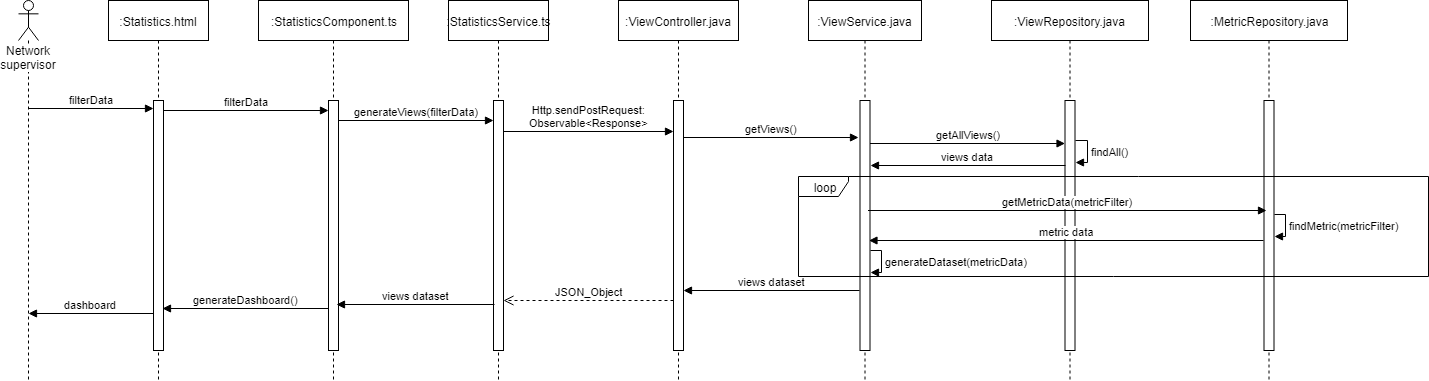
\includegraphics[width=17cm,height=10cm]{dashboardsequencediagram.png}
\caption{Sequence diagram of dashboard operation}
\label{fig:dashboardsequencediagram}
\end{figure}

The statistics and charts configuration consists of creating a model carrying a view configuration that we can use it to generate the same view each time. The statistics and charts management module contains two parts, the first one is the views configuration and the second one is the dashboard generation. 

To achieve creating customized views, from the presentation layer, Angular application, the user put the configuration he needs to generate the chart. This configuration goes through REST web service to the backend controller, then to the service layer. The service layer will take the view configuration as parameter to fetch the metrics data, stored in MongoDB, and process the received data in order create view dataset. The chart dataset goes through REST web service again to reach the frontend application arriving to the user interface. At this point, the user has the option to add this view to the dashboard, so the data.

The second part is the dashboard generation, when the user navigate to dashboard, there are three filters, time filter, location filter, and test filter. A request will be sent from the user interface and the Angular component and service to the backend through REST web service carrying the filters inputs. Views are fetched according to the test filter, and then the metrics data is fetched according location and time filter. The metrics data is processed to generate dataset for each view in the dashboard. Finally, the charts datasets goes back to the user interface.




\subsubsection{Authentication and users management module}
This module describes authentication and users accounts management process. This module is about creating, editing, deleting, and checking available users’ information.

The following class diagram (fig.\ref{fig:userclassdiagram}) presents the involved classes and components that build our module.

\begin{figure}[H]
\centering
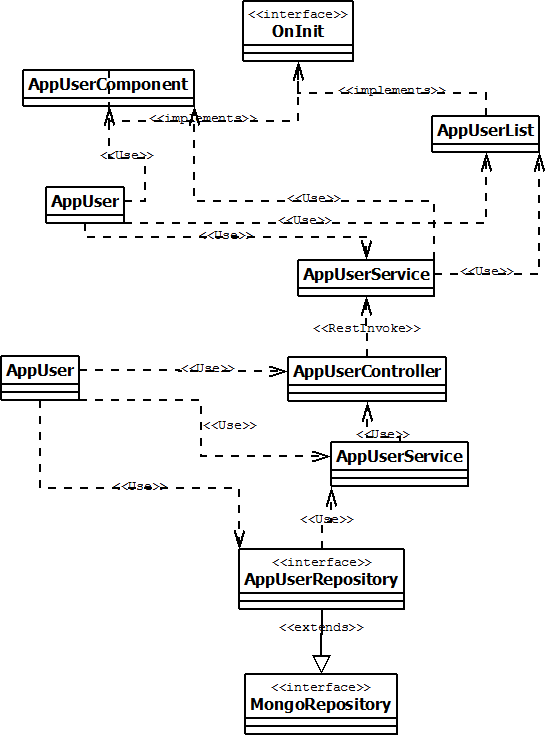
\includegraphics[width=15cm]{userclassdiagram.png}
\caption{Class diagram of the authentication and users management module}
\label{fig:userclassdiagram}
\end{figure}

Then, we have the sequence diagram that describes the interaction between the module components; this diagram presents the creation and updating users’ information operations:

\begin{figure}[H]
\centering
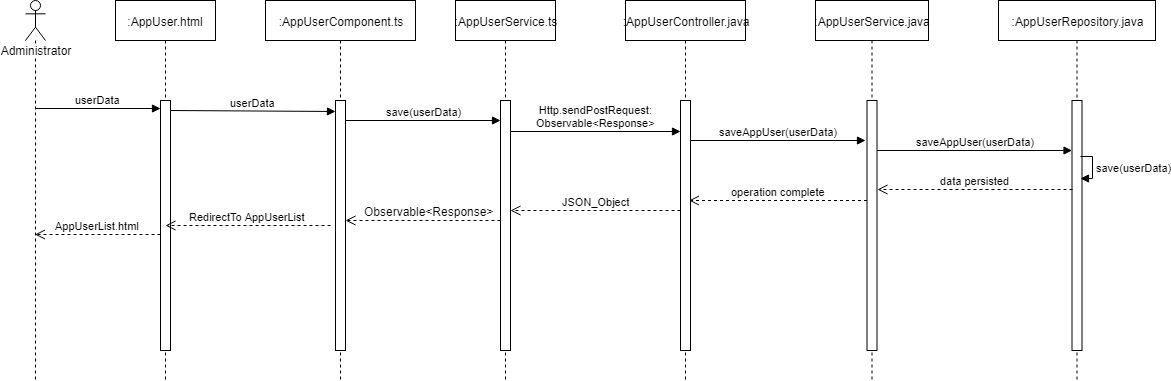
\includegraphics[width=17cm,height=10cm]{usersequencediagram.png}
\caption{Sequence diagram of users’ creation and updating operations}
\label{fig:usersequencediagram}
\end{figure}

The user configuration consists of creating a personalized user account that holds a username, a password, and a role or privilege.

The administrator just needs to fill the form with the user information. After finishing, a request is sent to the backend application in order to persist the user information. At this point, the user is able to authenticate.


\subsection{Broadband supervision and monitoring theory}
In the previous parts of the report we talked about the features offered by our solution concerning analytics and components management, although we did not emphasize the real-time network monitoring and metrics data processing. Also we need to clarify how the probes are handling tests and received configurations.

\paragraph{Tests and jobs handling between probes and Kafka}
~\\
We are using Kafka as mediator between the server and the probes. For every reboot, devices send their initial configuration to Kafka, in the counterpart, the devices receives their configurations, these configurations holds within it jobs and tests. The embedded application schedules the jobs using Crontab\cite{CRONTAB}. There a listener implemented on the boards in order to wait for configuration changes. The following (fig.\ref{fig:scriptskafka}) illustrates the interactions between a probe and Kafka. 

\begin{figure}[H]
\centering
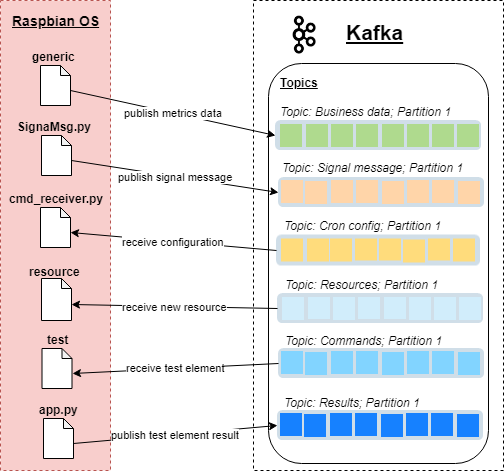
\includegraphics[width=15cm]{scriptskafka.png}
\caption{Device and Kafka interactions}
\label{fig:scriptskafka}
\end{figure}

\paragraph{Real-time processing and network monitoring}
~\\
As we mentioned earlier, after setting up the tests and alerts configurations, we have real-time data processing, this point is the crucial point of our solution. This part can decide the level of performance of the system. To achieve this task, we chose Kafka Stream.

Kafka Stream is a Kafka client that can handles real-time processing on data coming from a Kafka cluster or broker. Kafka stream subscribes to Business data topic, for each received test result, Kafka Stream brings the alerts configuration concerning the test in question, after, it tests the alerts constraints on the received data, if there is a satisfied constraint, it triggers a specific alert.

Another mission for Kafka Stream is to parse the received data in order to extract the metrics values to store it in MongoDB. However, between data parsing and storage, there is a specific processing for specific tests. In order to explain that, we should know that defining the quality of experience needs to have measurements from different timestamps with specific periods of time. To conclude, a complex calculation is required before storing data to have a better idea about the quality of experience.

Another crucial point in our solution, we need to have a high performance data analytics, MongoDB is an oriented document non-relational database that supports well indexing technique\cite{MONGODB}. MongoDB provides advanced querying operations that we used to perform our analytics with customized filters.




\section{Conclusion}
Through this chapter, we described each part of the solution, its functionalities both separately and when coordinating with other parts of the system. We also explained subsequently the choice of our logical and physical architecture. Concerning the detailed design, we exhibited the class and sequence diagram. In the next chapter, we present and expose the technologies employed during the process of the creation of our product.

\chapter{Project Achievements}

\section{Introduction}
In this chapter, we will discuss the process of implementing the different parts of the system. We start by presenting the different tools both software and hardware used in every task in order to complete the implementation process.

\section{Developing environment}
\subsection{Hardware envionment}
To achieve our project, we have used a DELL computer with a Windows 7 operating system. The characteristics of the used computer are provided below:
\begin{itemize}
\item	CPU: intel i5 2.3 Ghz
\item	RAM: 8 GB
\item	Hard Disk Drive: 500 GB
\end{itemize}
For the probes, we have used Raspberry Pi 3 B+ model with an embedded Raspbian operation system. The characteristics of the board are provided below:
\begin{itemize}
\item   CPU: 64-bit quad-core ARM v8
\item	RAM: 1 GB
\item	Memory card: 16 GB
\end{itemize}

\subsection{Software environment}
In this part, we list the software programs and applications we used throughout the development of our system.
\begin{itemize}
\item	Netbeans IDE 8.2: Netbeans is an integrated development environment developed by Oracle. Netbeans can be used with many programming languages; in our case we used it with Java programming language. Netbeans put in our hand many features to help developers achieving better coding performance.
\item	Visual studio code: Visual studio code is MIT open source licensed software, developed and maintained by Microsoft. It supports many programming languages with many different technologies just by integrating plugins within it. We used Visual studio code for Angular development. This software supports different platforms, Linux operation system, Windows, MacOS.
\item	Code Blocks IDE: Code Blocks is an integrated development environment for Fortan, C and C++ programming languages. We used it for C programming.  
\item	MongoDB: MongoDB is a non-relational database management system based in documents. It provides many advanced features like indexing and advanced operations algorithm to query on the documents. 	To generate analytics with high performance, we need a database that supports well indexes; also we need a database that provides different and flexible querying techniques like map and reduce algorithm. So the better choice for us was MongoDB.
\item	Apache Tomcat web server: Tomcat is a web server that supports Java web logic. In our case used an embedded Tomcat web server.
\item	Postman: Postman allows users to execute and build personalized HTTP requests; to achieve this Postman provides many optional features.
\item	Thonny: Thonny is an integrated development environment for Python programming language running on Raspbian operating system. We used it to develop our Python scripts.
\item	Geny: Geny is an integrated development environment that supports many programming languages. This software is running on Raspbian operating system. We used it to develop C programs on RaspBerry Pi board.
\end{itemize}

\subsection{Frameworks and technologies}
In this section, we discuss the technical choices we made to achieve our final product. We start by presenting the programming languages used in the development of the project. Afterwards, we defend our choice for the frameworks we used.
\paragraph{Programming languages}
~\\
\begin{itemize}
\item	Java: Java is a general purpose oriented object programming language. We used it to develop the backend of our solution.
\item	Typescript: Typescript is a programming language developed and maintained by Microsoft. Typescript is an object oriented programming language. We used it to develop our frontend application with Angular.
\item	Python: Python is a general purpose, high-level programming language. We used it in an embedded environment with Raspberry Pi boards.
\item	C: C is a procedural and a general purpose programming language. We used it in an embedded environment, with Raspberry Pi boards.
\item	Shell script: Shell script is a command line interpreter. We used it to install our embedded application.
\end{itemize}

\paragraph{Frameworks and technologies}
~\\
\begin{itemize}
\item	Spring framework: Spring is a Java application framework. Spring allows users to create enterprise services with POJO (Plain Old Java Objects). Spring uses dependency injection technique; also it provides many application configuration features.
\item	Spring data MongoDB: Spring data MongoDB is a part of Spring data project which aims to provide a Spring-based APIs (Application Programming Interfaces) for new datastores such as MongoDB. It gives the possibility to execute complex queries on MongoDB, especially with Mongo Template\cite{SPRINGDATAMONGODB}.
\item	Angular 7: Angular is an open source framework developed by Google. Angular is used for frontend application development, it gives the possibility to handle dynamically user interface. Angular is written entirely in Javascript, although it used Typescript as programming language.
\item	Apache Kafka: Kafka is distributed, fault-tolerant, horizontally scalable, wicked fast streaming platform. It is used for building real-time data pipelines and streaming applications with publish and subscribe technique. We used it as a middleware between widespread probes and the backend application.
\item	Kafka Stream: Kafka stream is a client library for building applications where the input and output data messages are stored in Kafka cluster or broker. It allows run real-time processing on the data. We used it for real-time processing.
•	Google protocol buffer: Protocol buffer is a protocol for structured data serializing, Protocol buffer, also known as Protobuf, supports several programming language such as Java, Objective-C, Python and C++.We used it to on the messages coming from the probes. We used this protocol because it is faster than the ordinary data format like JSON.
\item	OAuth 2.0: OAuth is a protocol for authorization flows for web application. It is simple for developers to use. We used it for security issues in our web application.
\item	Spring Security: Spring Security is a framework to build applications with powerful and highly customizable authentication and access control\cite{SPRINGSECURITY}.
\item	Linux Crontab: Crontab is a tool for job and task scheduling on Linux operating system, in our case Raspbian. We used it to schedule test running.
\item	MXparser: MXparser is a library for mathematical expressions parsing and evaluating. We used it with application features that need formula parsing such the case of alerting constraints.
\item	Bootstrap: Bootstrap is an open source frontend library created by Twitter for developing with HTML, CSS and Javascript in order to build responsive, mobile-first projects.
\end{itemize}


\section{Achieved work}
\subsection{Authentication and users management}
Before starting using the application features, an authentication is required; the figure below (fig.\ref{fig:login}) presents the login screen:
\begin{figure}[H]
\centering
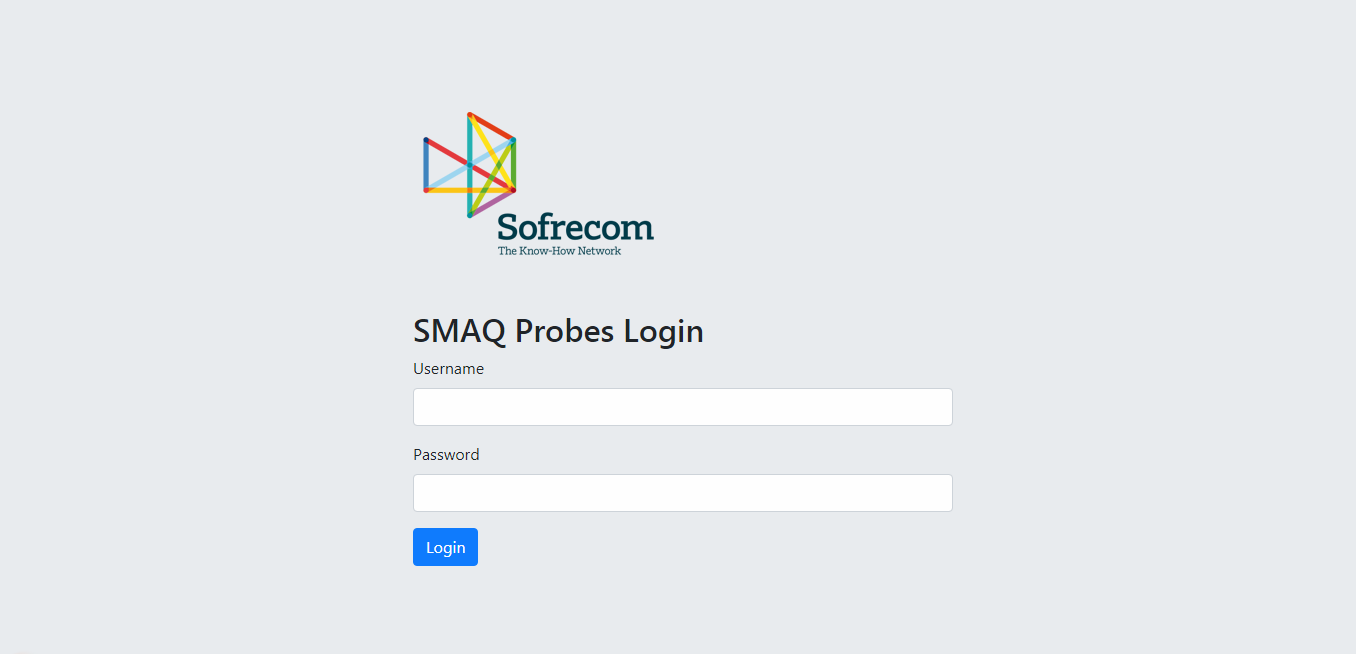
\includegraphics[width=15cm]{login.PNG}
\caption{Authentication screen}
\label{fig:login}
\end{figure}
The figure (fig.\ref{fig:users}) shows the users list with their information; this screen is only accessible from an administrator account:	
\begin{figure}[H]
\centering
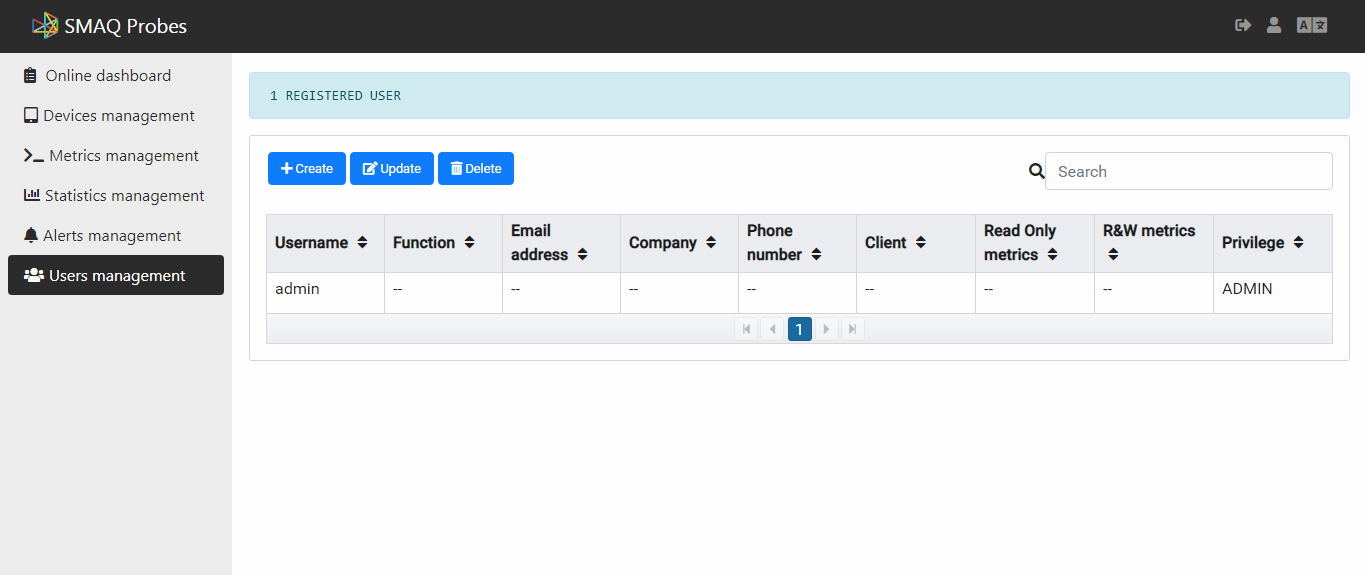
\includegraphics[width=15cm]{user.PNG}
\caption{Users list screen}
\label{fig:users}
\end{figure}
The figure (fig.\ref{fig:updateuser}) presents user information form, these screen is used for creating and updating users:
\begin{figure}[H]
\centering
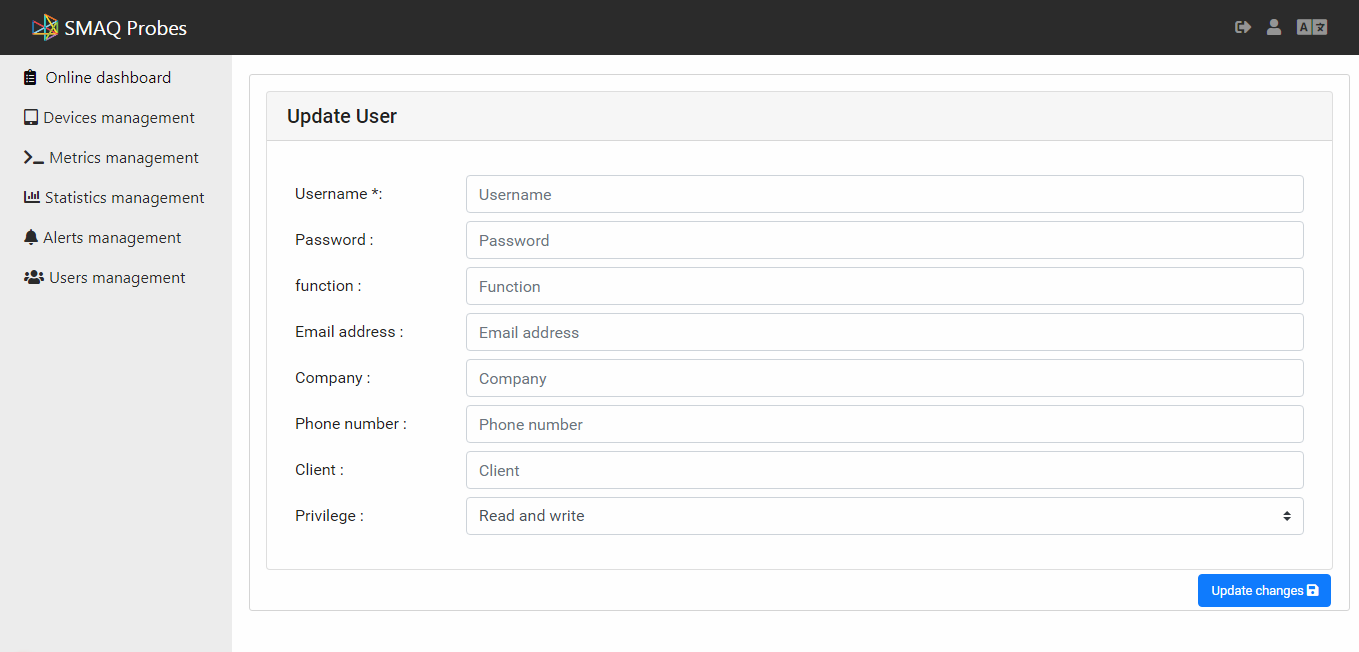
\includegraphics[width=15cm]{updateuser.PNG}
\caption{User updating screen}
\label{fig:updateuser}
\end{figure}



\subsection{Devices management}
As we said the devices module consists of connected devices information and jobs management, the following screen (fig.\ref{fig:device})  presents the devices information list:
\begin{figure}[H]
\centering
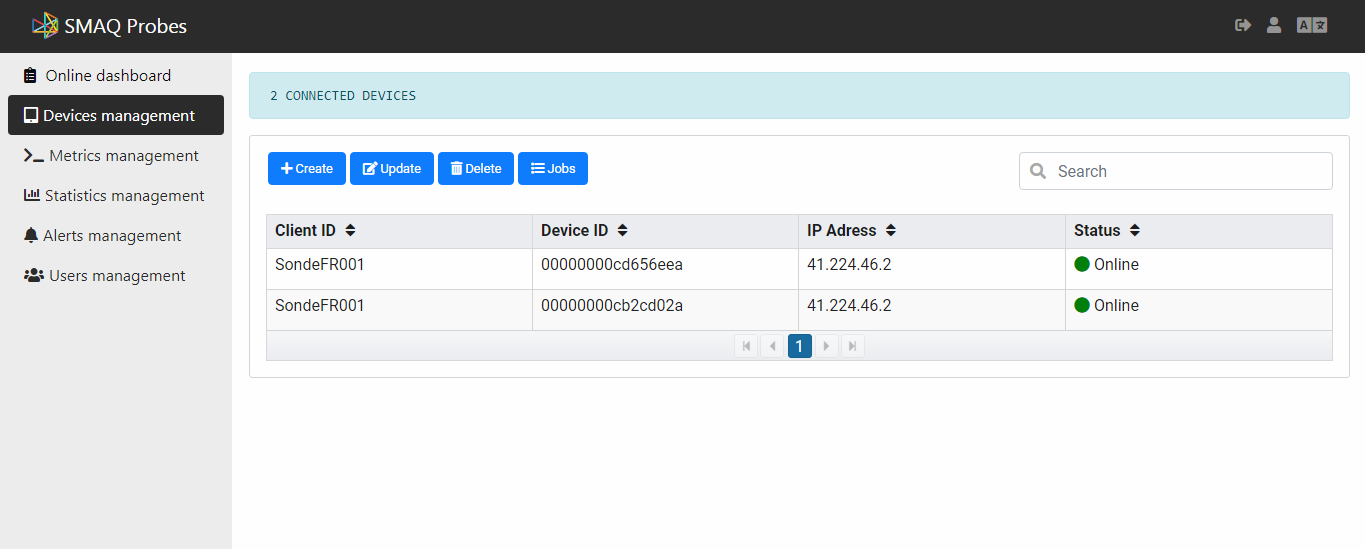
\includegraphics[width=15cm]{device.PNG}
\caption{Devices list screen}
\label{fig:device}
\end{figure}
As we can see we can navigate to jobs list using this screen.

The following figure (fig.\ref{fig:updatingdevice}) presents device updating screen:
\begin{figure}[H]
\centering
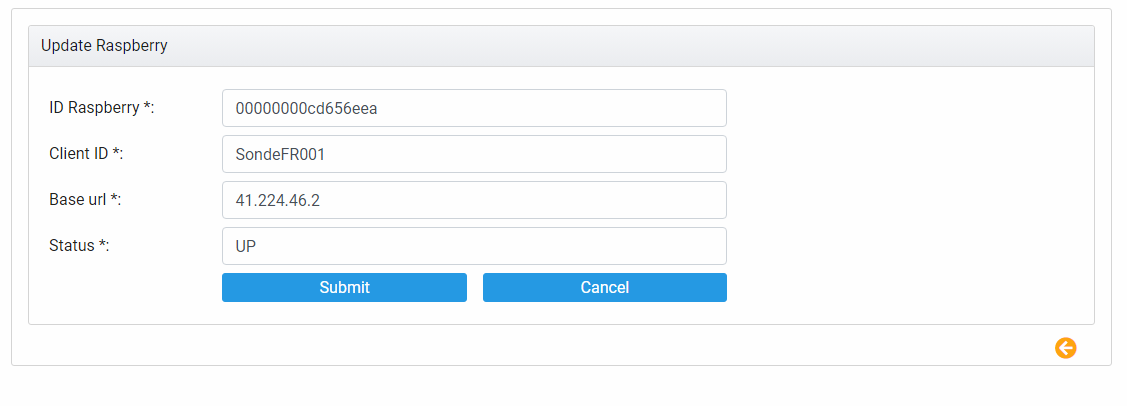
\includegraphics[width=15cm]{updatedevice.PNG}
\caption{Device updating screen}
\label{fig:updatingdevice}
\end{figure}
The second part of the device configuration is the jobs list, the following figure (fig.\ref{fig:cron}) presents the jobs list of a chosen device:
\begin{figure}[H]
\centering
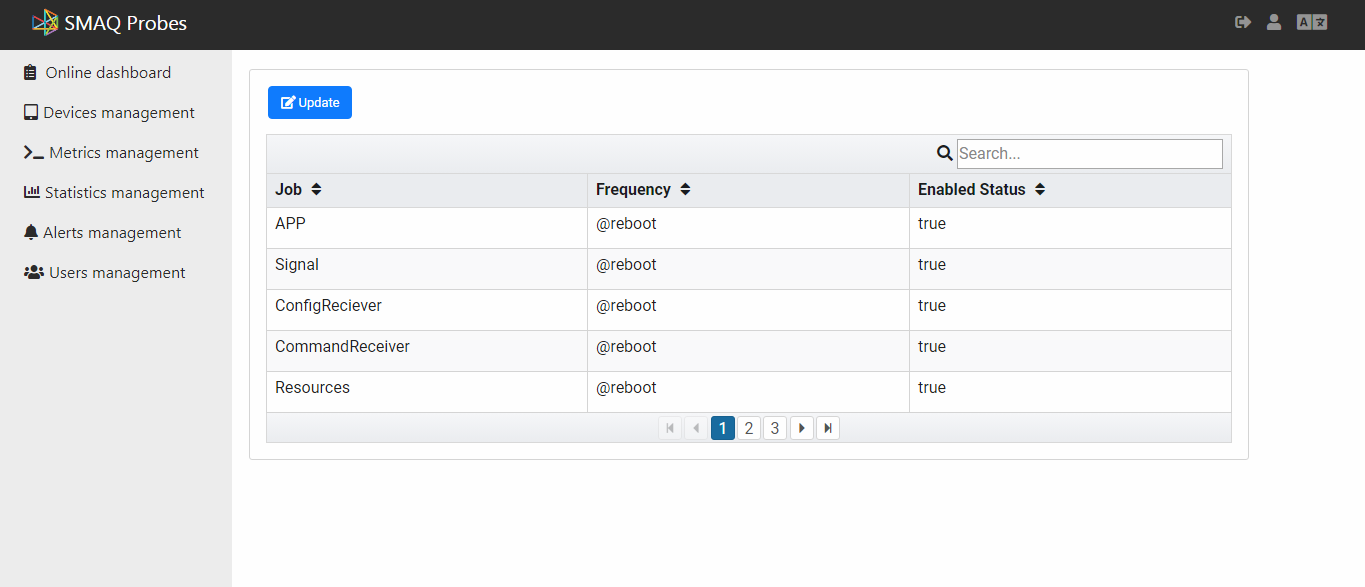
\includegraphics[width=15cm]{cron.PNG}
\caption{Crons list screen}
\label{fig:cron}
\end{figure}
Next, this figure (fig.\ref{fig:updatingcron}) describes the job updating operation, as we can see we change the schedules using this screen:
\begin{figure}[H]
\centering
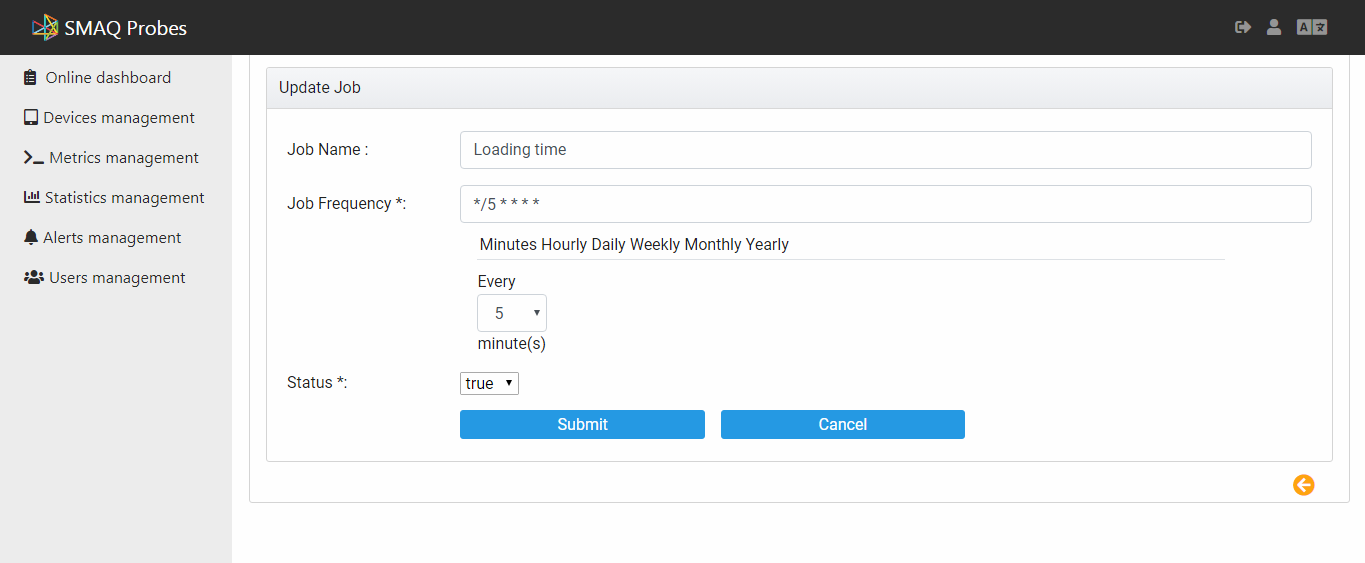
\includegraphics[width=15cm]{updatecron.PNG}
\caption{Cron updating screen}
\label{fig:updatingcron}
\end{figure}
After submitting this form, the new configuration will be sent to the device in question.





\subsection{Metrics and tests management}
Metrics and test management module is responsible for creating tests for the probes; the following screen (fig.\ref{fig:metric}) shows the tests list:
\begin{figure}[H]
\centering
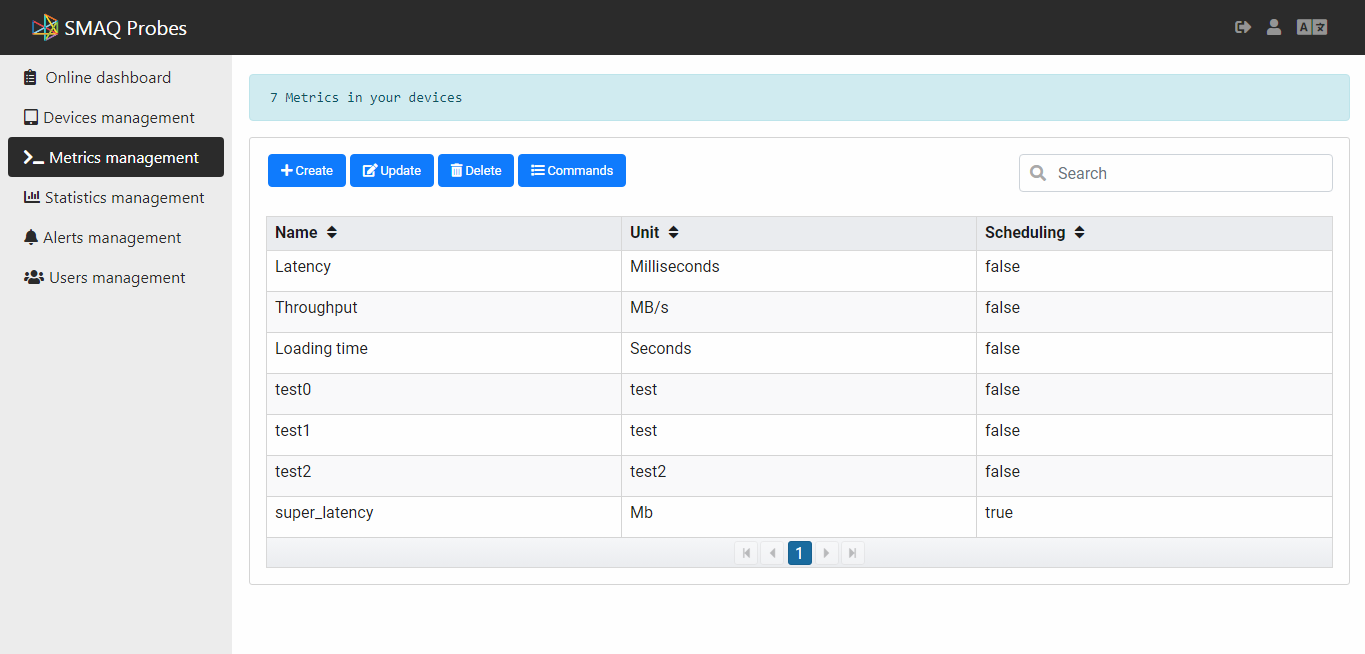
\includegraphics[width=15cm]{metric.PNG}
\caption{Tests list screen}
\label{fig:metric}
\end{figure}
To update or create a test, we have this wizard (fig.\ref{fig:wizard}):
\begin{figure}[H]
\centering
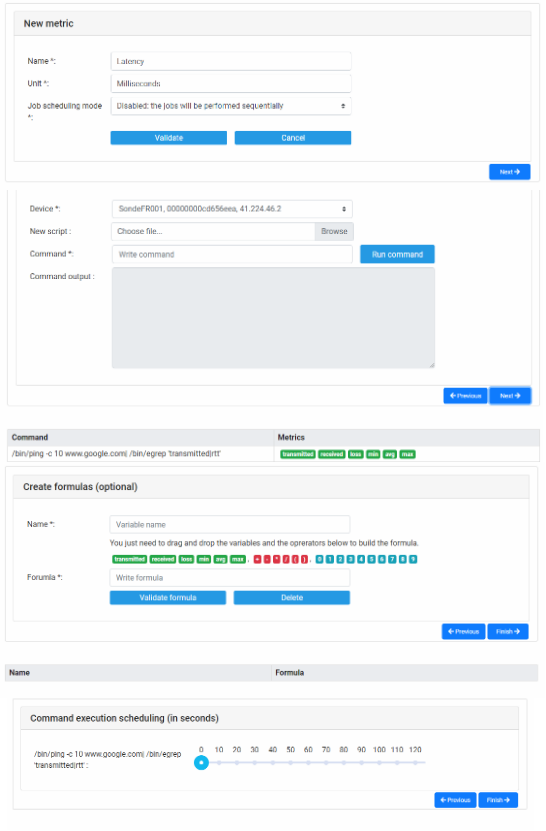
\includegraphics[width=15cm]{wizard.png}
\caption{Test configuring wizard screen}
\label{fig:wizard}
\end{figure}
With this wizard we can create test elements that contain formulas; also we can add new resources to the devices and create test element schedules, and of course we can test each element directly on a connected device.




\subsection{Alerts management}
The network monitoring module consists of creating alerts with customized constraints. The following figure (fig.\ref{fig:alert}) presents the alerts list.
\begin{figure}[H]
\centering
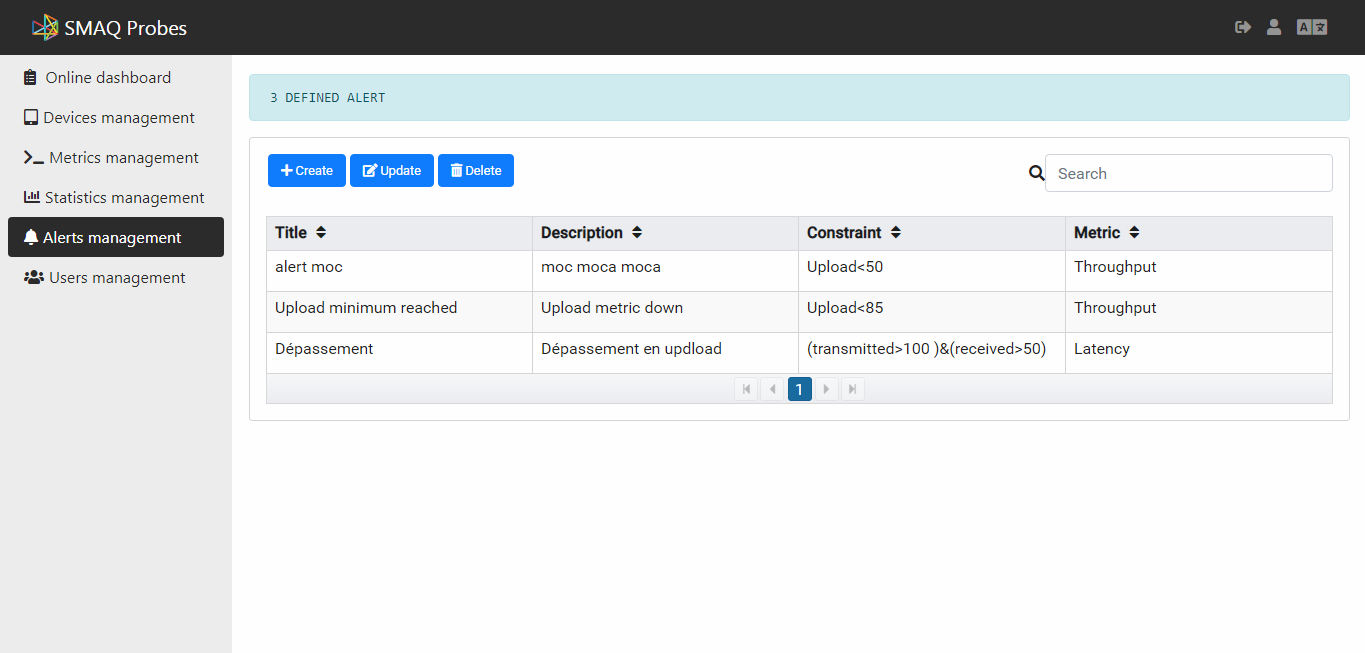
\includegraphics[width=15cm]{alert.PNG}
\caption{Alerts list screen}
\label{fig:alert}
\end{figure}
The following form (fig.\ref{fig:createalert}) illustrates alerts creation. The constraint field must have a logic expression as input. To facilitate the task we are using drag and drop module with personalized elements:
\begin{figure}[H]
\centering
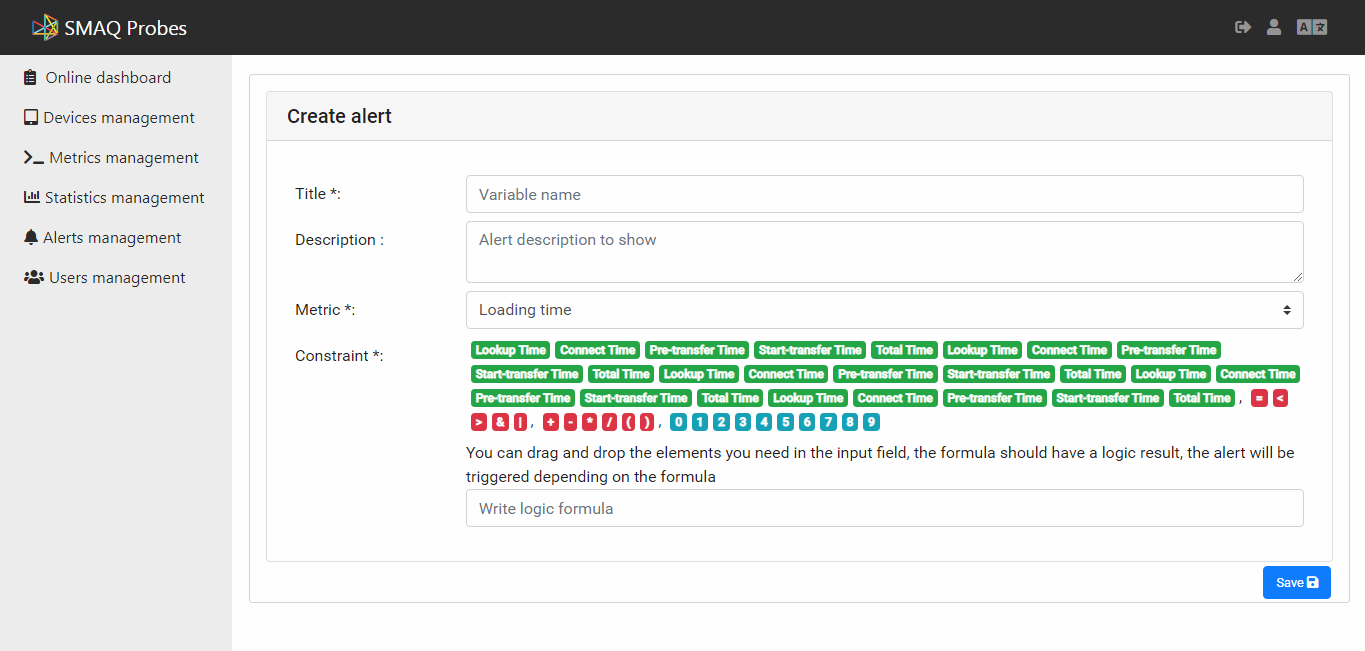
\includegraphics[width=15cm]{createalert.PNG}
\caption{Alert configuring screen}
\label{fig:createalert}
\end{figure}




\subsection{Statistics and dashboard management}
The statistics and dashboard management module consists of testing and creating customized charts to be visualized by network supervisors on the dashboard. The following figure (fig.\ref{fig:statistic}) presents the chart generation process:
\begin{figure}[H]
\centering
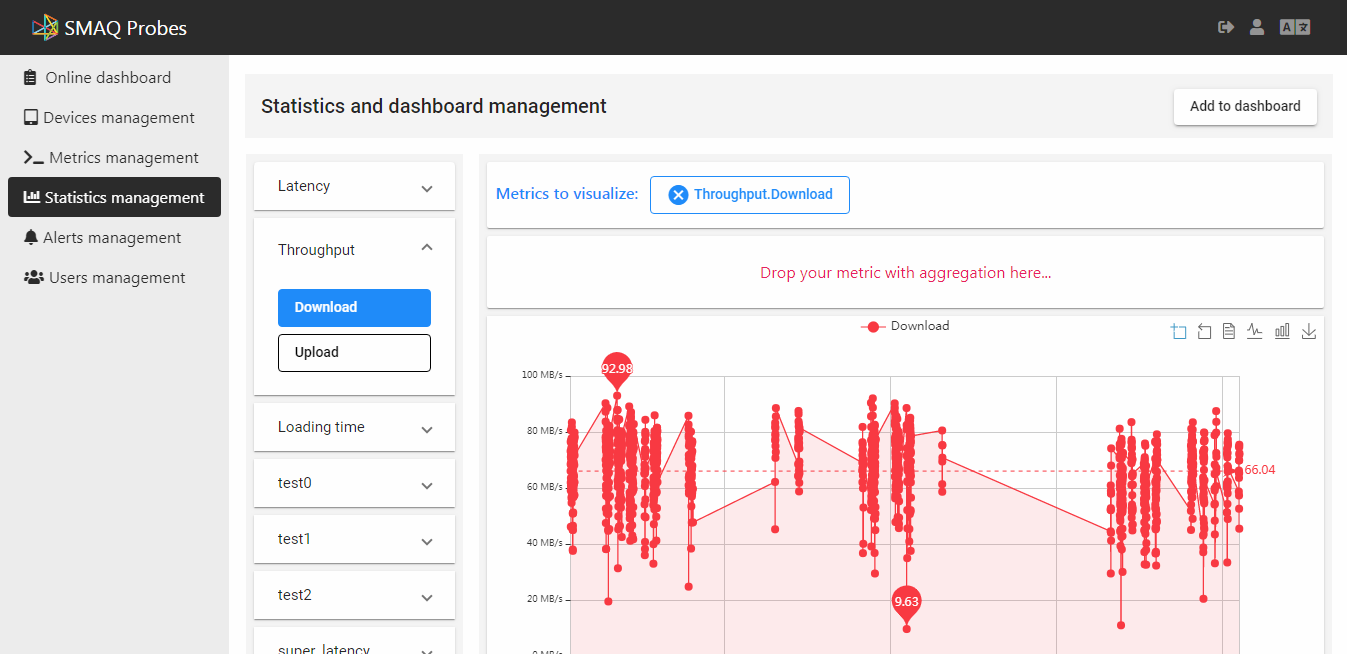
\includegraphics[width=15cm]{statistics.PNG}
\caption{Chart customizing screen}
\label{fig:statistic}
\end{figure}
At this point the user has the right to ass this view to the dashboard.

Last but not least we have our dashboard. The figure (fig.\ref{fig:dashboard}) presents an overview of the dashboard:
\begin{figure}[H]
\centering
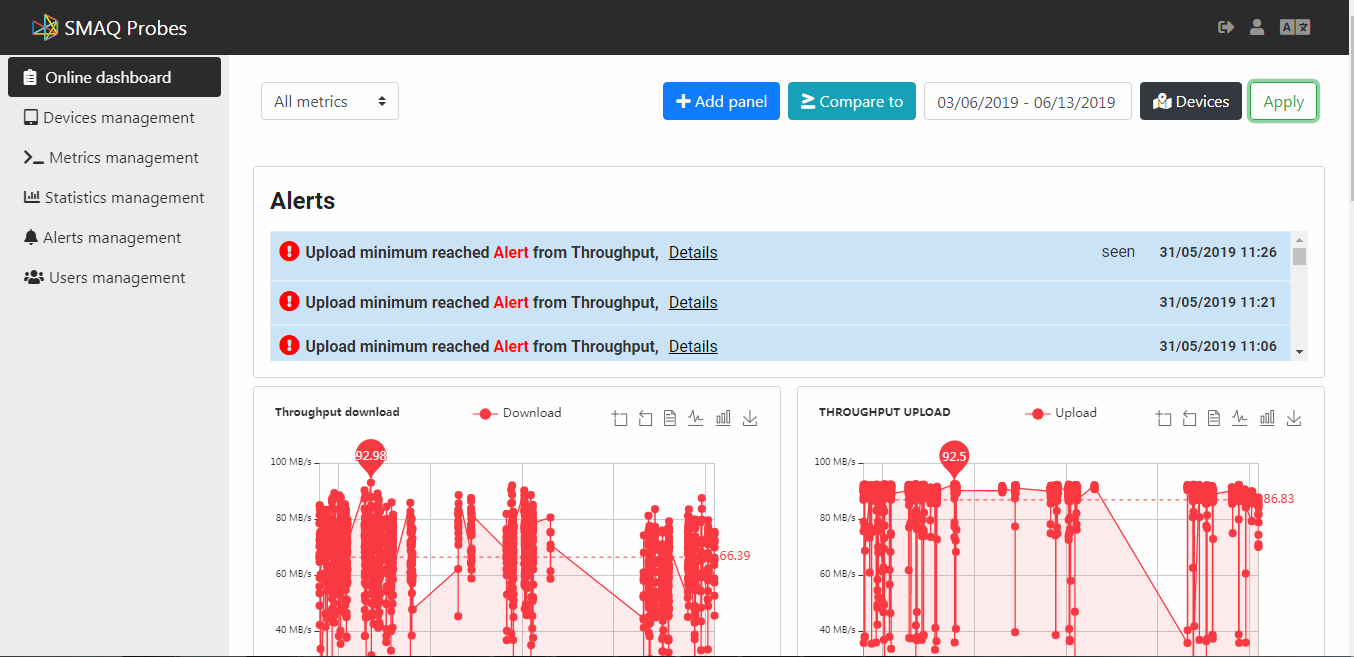
\includegraphics[width=15cm]{dashboard.PNG}
\caption{Online dashboard screen}
\label{fig:dashboard}
\end{figure}
The following filters are already implemented in the dashboard. The following screen (fig.\ref{fig:timefilter}) presents the time period filter:
\begin{figure}[H]
\centering
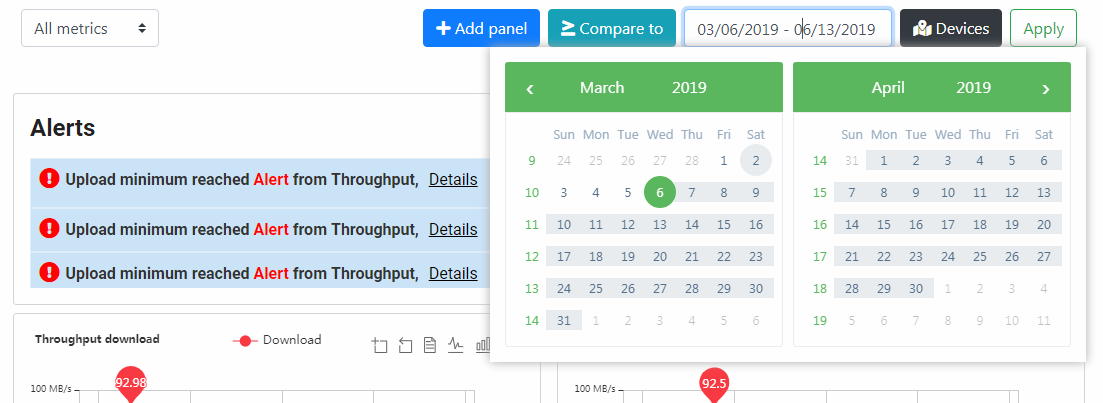
\includegraphics[width=15cm]{timefilter.PNG}
\caption{Time period filter}
\label{fig:timefilter}
\end{figure}
The following figure (fig.\ref{fig:locationfilter}) presents the location filter. This filter gives the hand to users to get the charts according zone area:
\begin{figure}[H]
\centering
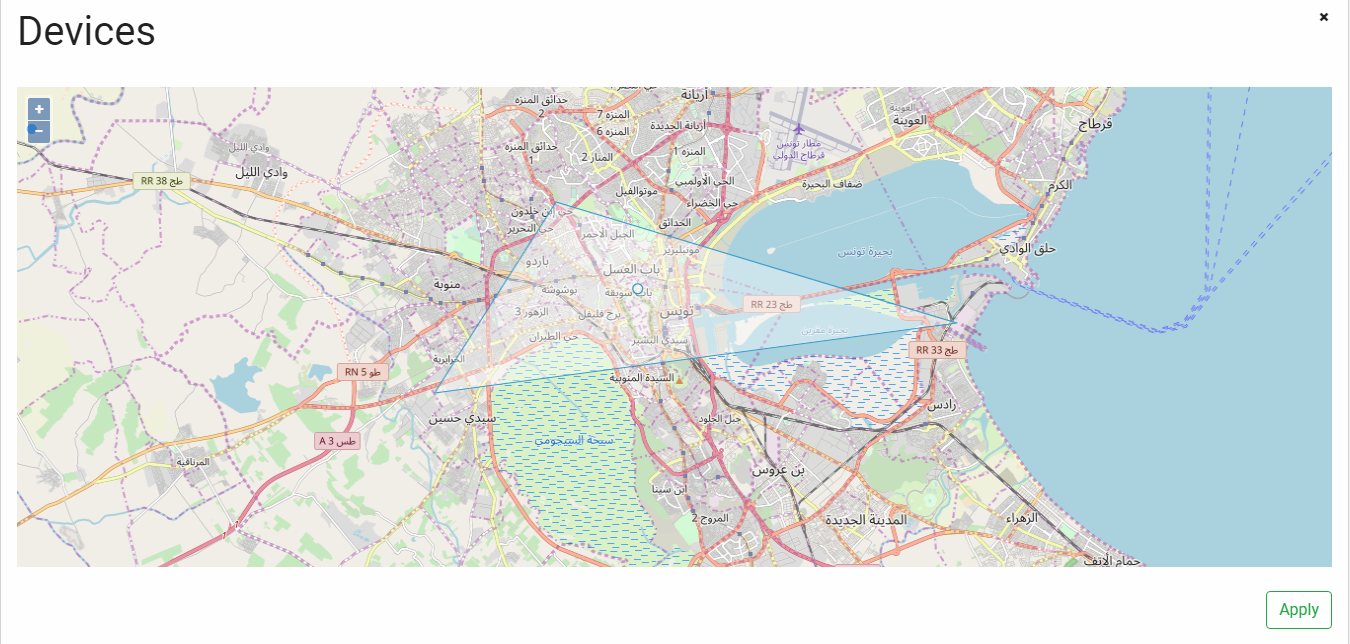
\includegraphics[width=15cm]{locationfilter.PNG}
\caption{Devices filter}
\label{fig:locationfilter}
\end{figure}
To give the user more information about the quality of experience, we implemented a comparison filters that generates charts to compare between periods and zones (fig.\ref{fig:comparingfilter}):
\begin{figure}[H]
\centering
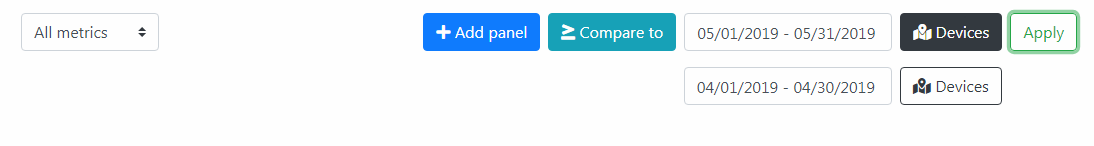
\includegraphics[width=15cm]{comparingfilter.PNG}
\caption{Comparison filters}
\label{fig:comparingfilter}
\end{figure}
A part of the dashboard is reserved for alerts. The user can access to an alert details as follows in (fig.\ref{fig:alertdetail}):
\begin{figure}[H]
\centering
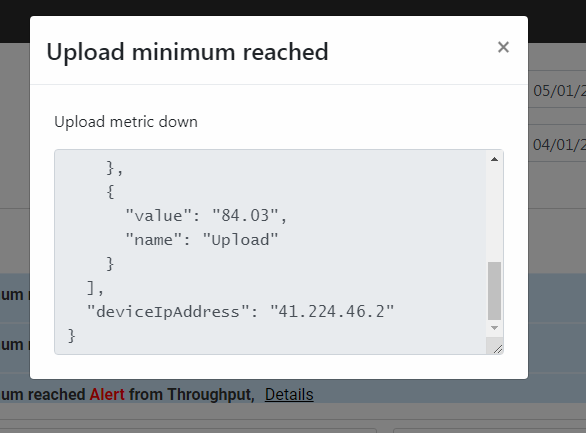
\includegraphics[width=15cm]{alertdetail.PNG}
\caption{Triggered alert detail screen}
\label{fig:alertdetail}
\end{figure}
The charts that we are using in dashboard have several advanced options like data zooming, data visualizing and bar chart support\cite{ECHARTS}. The following figure fig.\ref{fig:chart}) is a sample:
\begin{figure}[H]
\centering
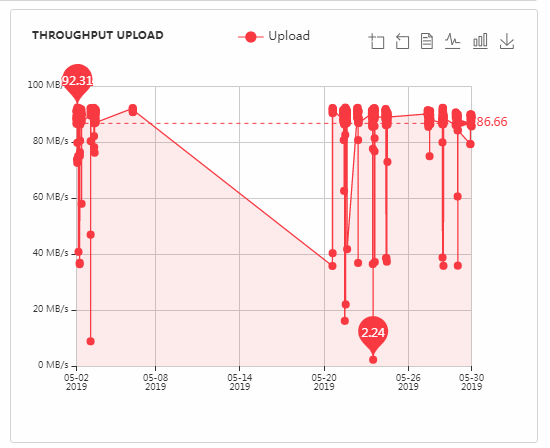
\includegraphics[width=15cm]{charts.PNG}
\caption{Implemented chart}
\label{fig:chart}
\end{figure}



\section{Conclusion}
uring this chapter, we presented the technologies that were chosen to implement our project and we argued that choice. We also presented the used frameworks and we finished by displaying the main features and interfaces of our components.

\chapter{General Conclusion and Future Work}
We were focused on solving the broadband supervision and monitoring issue by designing and developing a flexible and easy-to-use platform. As a matter of fact, we implemented a web application that helps network supervisors to assess the quality of service of their networks. This information (quality of service) is provided by data analytics, this data is coming from widespread probes. We designed the platform in order to give users the flexibility they need to manage their tests and devices online.

For the graphic user interface, we developed many advanced graphic options to give users better experience with our application.

During the project, we were aware of data security, so we implemented many security techniques. 

As every project can be enhanced and expanded, various perspectives are imminent for our project. We can mention the enhancement of the real-time processing component using machine learning algorithms to predict the quality of experience, there is some technologies that can be integrated with our platform in order to achieve these enhancements. With this empowering we can predict unusual quality of experience.


\begin{thebibliography}{9}
\bibitem{SAMKNOWS} 
SamKnows. \\
\textit{Samknows tests}. \\
\href{https://samknows.com/technology/tests}{https://samknows.com/technology/tests}.



\bibitem{SPRINGDATAMONGODB}  
Mark Pollack,
Thomas Risberg,
Oliver Gierke,
Costin Leau,
Jon Brisbin,
Thomas Darimont,
Christoph Strobl,
Mark Paluch,
Jay Bryant.
\\
\textit{Spring Data MongoDB - Reference Documentation}\\
\href{https://docs.spring.io/spring-data/mongodb/docs/current/reference/html/}{https://docs.spring.io/spring-data/mongodb/docs/current/reference/html/}.


\bibitem{KAFKASTREAM} 
Apache Sotware Foundation. \\
\textit{Kafka Streams
}. \\
\href{https://docs.confluent.io/current/streams/index.html}
{https://docs.confluent.io/current/streams/index.html}.



\bibitem{RDKAFKA} 
edenhill Github. \\
\textit{librdkafka the Apache Kafka C/C++ client library
}. \\
\href{https://docs.confluent.io/2.0.0/clients/librdkafka/index.html}
{https://docs.confluent.io/2.0.0/clients/librdkafka/index.html}.


\bibitem{SPRINGSECURITY} 
Eugen Paraschiv. \\
\textit{Using JWT with Spring Security OAuth
}. \\
\href{https://www.baeldung.com/spring-security-oauth-jwt}
{https://www.baeldung.com/spring-security-oauth-jwt}.



\bibitem{MONGODB} 
MongoDB. \\
\textit{Indexes
}. \\
\href{https://docs.mongodb.com/manual/indexes/}
{https://docs.mongodb.com/manual/indexes/}.


\bibitem{ECHARTS} 
ECHARTS Community. \\
\textit{ECHARTS
}. \\
\href{https://echarts.apache.org/en/index.html}
{https://echarts.apache.org/en/index.html}.


\bibitem{ANGULAR} 
 Google. \\
\textit{Angular 7
}. \\
\href{https://v7.angular.io/docs}
{https://v7.angular.io/docs}.


\bibitem{CRONTAB} 
 Python community. \\
\textit{python-crontab 2.3.6
}. \\
\href{https://pypi.org/project/python-crontab/}
{https://pypi.org/project/python-crontab/}.

\end{thebibliography}

%\chapter*{Appendix}

\end{document}
